\documentclass[a4paper,10pt]{article}
\usepackage[utf8]{inputenc}
\usepackage{graphicx}
\usepackage{booktabs}
\usepackage{longtable}
\usepackage{rotating}
\usepackage{subfigure}
\usepackage{multirow}
\usepackage{amssymb}
\usepackage{indentfirst}
\usepackage{float}
\usepackage{url}
\usepackage{cite}
\usepackage{amsmath}
\usepackage{xcite} % Cite stuff from the main text
\usepackage{xr} % automatic cross-referencing
\usepackage[authoryear,round]{natbib}
\bibliographystyle{apalike}
%%% Supp Mat modifications
\renewcommand\refname{Further References}
\externaldocument{FMDV_AMERICA}
\externalcitedocument[M-]{FMDV_AMERICA}
\renewcommand{\thesubfigure}{(\Alph{subfigure})}
\renewcommand{\thetable}{S\arabic{table}}   
\renewcommand{\thefigure}{S\arabic{figure}}

%%%%%
\topmargin 0.0cm
\oddsidemargin 0.5cm
\evensidemargin 0.5cm
\textwidth 16cm
\textheight 21cm
\pagestyle{myheadings}
%%%%%
%opening
\title{Text S2 -- Supplementary information to ``Spatio-temporal Dynamics of Foot-and-Mouth Disease Virus in South America''}
\author{
Luiz Max Carvalho, Nuno Rodrigues Faria, Andres Perez,
Marc A. Suchard, Philippe Lemey,\\
Waldemir de Castro Silveira,\\
Andrew Rambaut and Guy Baele
}

\date{June, 2019}
\begin{document}

\maketitle

\section*{Data collection and curation}

In Tables~\ref{stab:sequences_A} and~\ref{stab:sequences_O} we provide the GenBank accession numbers, date and country of collection of all sequences used in this study.

\begin{center}
 \begin{longtable}{ccc}
  \caption{\textbf{Accession numbers, date and country of collection for the serotype A sequences}. When only the year of collection was known, we used the 15th of July as the collection date.}
  \label{stab:sequences_A} \\

\hline \multicolumn{1}{|c|}{\textbf{Accession}} & \multicolumn{1}{c|}{\textbf{Date}} & \multicolumn{1}{c|}{\textbf{Country}} \\ \hline 
\endfirsthead

\multicolumn{3}{c}%
{{\bfseries \tablename\ \thetable{} -- continued from previous page}} \\
\hline \multicolumn{1}{|c|}{\textbf{Accession}} & \multicolumn{1}{c|}{\textbf{Date}} & \multicolumn{1}{c|}{\textbf{Country}} \\ \hline 
\endhead

\hline \multicolumn{3}{|r|}{{Continued on next page}} \\ \hline
\endfoot

\hline \hline
\endlastfoot
JQ082960 & 1955-07-15 & Brazil \\
AJ306222 & 1955-07-15 & Argentina \\
AJ251476 & 1955-07-15 & Brazil \\
AY593768 & 1955-07-15 & Brazil \\
JQ082955 & 1958-07-15 & Brazil \\
AY593788 & 1958-07-15 & Brazil \\
AY593753 & 1958-07-15 & Brazil \\
JQ082961 & 1959-07-15 & Argentina \\
JQ082956 & 1959-07-15 & Brazil \\
JQ082957 & 1959-07-15 & Brazil \\
AY593769 & 1959-07-15 & Argentina \\
AY593756 & 1959-07-15 & Brazil \\
AY593789 & 1961-07-15 & Argentina \\
JQ082958 & 1962-07-15 & Venezuela \\
JQ082959 & 1962-07-15 & Argentina \\
AY593767 & 1965-07-15 & Argentina \\
JQ082962 & 1966-07-15 & Argentina \\
AY593770 & 1966-07-15 & Argentina \\
JQ082963 & 1967-07-15 & Colombia \\
AY593757 & 1967-07-15 & Brazil \\
AY593771 & 1967-07-15 & Colombia \\
AY593758 & 1967-07-15 & Venezuela \\
AJ308694 & 1968-07-15 & Argentina \\
AY593801 & 1968-07-15 & Uruguay \\
JQ082964 & 1969-07-15 & Peru \\
AY593773 & 1969-07-15 & Peru \\
JQ082965 & 1970-07-15 & Venezuela \\
JQ082966 & 1970-07-15 & Brazil \\
EU553882 & 1970-07-15 & Venezuela \\
AY593775 & 1970-07-15 & Venezuela \\
AJ306220 & 1971-07-15 & Argentina \\
AJ308695 & 1971-07-15 & Argentina \\
JQ082967 & 1975-07-15 & Ecuador \\
JQ082968 & 1975-07-15 & Peru \\
AJ409219 & 1976-07-15 & Argentina \\
EU553851 & 1976-07-15 & Brazil \\
JQ082969 & 1976-07-15 & Brazil \\
JQ082970 & 1976-07-15 & Brazil \\
JQ082971 & 1976-07-15 & Brazil \\
JQ082972 & 1976-07-15 & Colombia \\
APHA76 & 1976-07-15 & Venezuela \\
AY593787 & 1977-07-15 & Brazil \\
JQ082973 & 1979-07-15 & Ecuador \\
APHA79 & 1979-07-15 & Venezuela \\
AY593803 & 1979-07-15 & Brazil \\
KF112899 & 1981-07-15 & Argentina \\
JQ082974 & 1981-07-15 & Brazil \\
AJ306219 & 1981-07-15 & Argentina \\
JQ082975 & 1984-07-15 & Brazil \\
JQ082976 & 1984-07-15 & Colombia \\
JQ082977 & 1985-07-15 & Colombia \\
AY593794 & 1985-07-15 & Colombia \\
AJ306221 & 1987-07-15 & Argentina \\
JQ082978 & 1989-07-15 & Venezuela \\
AJ308698 & 1990-07-15 & Argentina \\
AJ308696 & 1990-07-15 & Argentina \\
AJ308697 & 1990-07-15 & Argentina \\
AJ308699 & 1991-07-15 & Argentina \\
AJ308702 & 1992-07-15 & Argentina \\
AJ308700 & 1992-07-15 & Argentina \\
AJ308701 & 1992-07-15 & Argentina \\
JQ082982 & 1997-07-15 & Brazil \\
JQ082979 & 1997-07-15 & Colombia \\
JQ082980 & 1997-07-15 & Colombia \\
JQ082981 & 1997-07-15 & Colombia \\
JQ082931 & 1999-07-15 & Peru \\
JQ082915 & 2000-05-30 & Bolivia \\
AY593782 & 2000-07-15 & Argentina \\
JQ082930 & 2000-07-15 & Peru \\
JQ082906 & 2000-08-15 & Argentina \\
AM179990 & 2000-08-15 & Argentina \\
AM179989 & 2000-08-15 & Argentina \\
AM179992 & 2000-08-15 & Argentina \\
AM179988 & 2000-08-15 & Argentina \\
AM179991 & 2000-08-15 & Argentina \\
AM179993 & 2000-08-15 & Argentina \\
AM179995 & 2000-09-15 & Argentina \\
AM179996 & 2000-09-15 & Argentina \\
AM179994 & 2000-09-15 & Argentina \\
AM179998 & 2000-10-15 & Argentina \\
AM179997 & 2000-10-15 & Argentina \\
AM179999 & 2000-11-15 & Argentina \\
JQ082937 & 2000-12-09 & Venezuela \\
KX002194 & 2000-12-31 & Argentina \\
KX002195 & 2001-02-10 & Argentina \\
KX002196 & 2001-02-18 & Argentina \\
KX002204 & 2001-03-07 & Argentina \\
KX002203 & 2001-03-13 & Argentina \\
JQ082907 & 2001-03-15 & Argentina \\
JQ082908 & 2001-03-15 & Argentina \\
JQ082909 & 2001-03-15 & Argentina \\
AM180007 & 2001-03-15 & Argentina \\
AM180000 & 2001-03-15 & Argentina \\
AM180005 & 2001-03-15 & Argentina \\
AM180008 & 2001-03-15 & Argentina \\
AM180002 & 2001-03-15 & Argentina \\
AM180006 & 2001-03-15 & Argentina \\
AM180001 & 2001-03-15 & Argentina \\
AM180003 & 2001-03-15 & Argentina \\
AM180004 & 2001-03-15 & Argentina \\
KX002178 & 2001-03-21 & Argentina \\
KX002205 & 2001-03-27 & Argentina \\
KX002193 & 2001-03-29 & Argentina \\
AM180009 & 2001-04-15 & Argentina \\
AM180014 & 2001-04-15 & Argentina \\
AM180010 & 2001-04-15 & Argentina \\
AM180012 & 2001-04-15 & Argentina \\
AM180013 & 2001-04-15 & Argentina \\
AM180015 & 2001-04-15 & Argentina \\
AM180011 & 2001-04-15 & Argentina \\
AM180016 & 2001-04-15 & Argentina \\
JQ082910 & 2001-04-15 & Uruguay \\
JQ082911 & 2001-04-15 & Uruguay \\
KX002198 & 2001-04-20 & Argentina \\
JQ082916 & 2001-05-07 & Bolivia \\
JQ082917 & 2001-05-10 & Bolivia \\
KX002200 & 2001-05-12 & Argentina \\
KX002201 & 2001-05-15 & Argentina \\
KX002202 & 2001-05-15 & Argentina \\
AM180019 & 2001-05-15 & Argentina \\
AM180017 & 2001-05-15 & Argentina \\
AM180018 & 2001-05-15 & Argentina \\
JQ082912 & 2001-05-15 & Brazil \\
JQ082913 & 2001-05-15 & Brazil \\
JQ082914 & 2001-05-15 & Brazil \\
KX002176 & 2001-05-25 & Argentina \\
KX002177 & 2001-05-28 & Argentina \\
KX002180 & 2001-06-03 & Argentina \\
JQ082918 & 2001-06-07 & Bolivia \\
JQ082932 & 2001-06-13 & Venezuela \\
AM180020 & 2001-06-15 & Argentina \\
AM180021 & 2001-06-15 & Argentina \\
KX002181 & 2001-06-16 & Argentina \\
KX002182 & 2001-06-17 & Argentina \\
KX002183 & 2001-06-17 & Argentina \\
KX002184 & 2001-07-10 & Argentina \\
AY593802 & 2001-07-15 & Uruguay \\
AY593783 & 2001-07-15 & Argentina \\
AY593784 & 2001-07-15 & Argentina \\
AY593785 & 2001-07-15 & Argentina \\
AY593786 & 2001-07-15 & Argentina \\
AY593790 & 2001-07-15 & Argentina \\
KX002186 & 2001-07-20 & Argentina \\
JQ082919 & 2001-07-23 & Bolivia \\
KX002185 & 2001-08-07 & Argentina \\
JQ082920 & 2001-08-07 & Bolivia \\
KX002189 & 2001-08-08 & Argentina \\
KX002188 & 2001-08-15 & Argentina \\
KX002187 & 2001-08-21 & Argentina \\
KX002191 & 2001-10-11 & Argentina \\
AM180022 & 2001-10-15 & Argentina \\
KX002192 & 2001-11-15 & Argentina \\
JQ082933 & 2001-12-15 & Venezuela \\
AM180024 & 2002-01-15 & Argentina \\
JQ082921 & 2002-03-30 & Bolivia \\
JQ082929 & 2002-06-15 & Ecuador \\
JQ082934 & 2002-11-28 & Venezuela \\
JQ082935 & 2003-05-14 & Venezuela \\
JQ082936 & 2003-07-03 & Venezuela \\
JQ082938 & 2003-12-12 & Venezuela \\
JQ082939 & 2004-01-23 & Venezuela \\
JQ082940 & 2004-02-11 & Venezuela \\
JQ082941 & 2004-03-10 & Venezuela \\
JQ082942 & 2004-04-01 & Venezuela \\
JQ082943 & 2004-05-19 & Venezuela \\
JQ082944 & 2004-07-12 & Venezuela \\
JQ082922 & 2004-07-15 & Colombia \\
JQ082945 & 2004-08-13 & Venezuela \\
JQ082946 & 2004-08-26 & Venezuela \\
JQ082947 & 2004-09-24 & Venezuela \\
JQ082948 & 2004-11-18 & Venezuela \\
JQ082949 & 2005-02-03 & Venezuela \\
JQ082950 & 2005-04-06 & Venezuela \\
JQ082951 & 2005-04-20 & Venezuela \\
JQ082952 & 2005-04-29 & Venezuela \\
JQ082953 & 2006-06-13 & Venezuela \\
JQ082954 & 2007-01-30 & Venezuela \\
JQ082923 & 2008-06-06 & Colombia \\
JQ082924 & 2008-06-06 & Colombia \\
JQ082925 & 2008-06-06 & Colombia \\
JQ082926 & 2008-06-06 & Colombia \\
JQ082927 & 2008-06-06 & Colombia \\
JQ082928 & 2008-06-06 & Colombia \\
KU234721 & 2013-04-01 & Venezuela
 \end{longtable}
\end{center}

\begin{center}
 \begin{longtable}{ccc}
  \caption{\textbf{Acession numbers, date and country of collection for the serotype O sequences}. When only the year of collection was known, we used the 15th of July as the collection date.}
  \label{stab:sequences_O} \\

\hline \multicolumn{1}{|c|}{\textbf{Accession}} & \multicolumn{1}{c|}{\textbf{Date}} & \multicolumn{1}{c|}{\textbf{Country}} \\ \hline 
\endfirsthead

\multicolumn{3}{c}%
{{\bfseries \tablename\ \thetable{} -- continued from previous page}} \\
\hline \multicolumn{1}{|c|}{\textbf{Acession}} & \multicolumn{1}{c|}{\textbf{Date}} & \multicolumn{1}{c|}{\textbf{Country}} \\ \hline 
\endhead

\hline \multicolumn{3}{|r|}{{Continued on next page}} \\ \hline
\endfoot

\hline \hline
\endlastfoot
APHVP1OC & 1971-07-15 & Brazil \\
AY593827 & 1971-07-15 & Venezuela \\
AJ308705 & 1977-07-15 & Argentina \\
DQ789075 & 1983-07-15 & Argentina \\
AJ308706 & 1983-07-15 & Argentina \\
KJ831663 & 1990-07-15 & Bolivia \\
AJ308707 & 1990-07-15 & Argentina \\
KJ831741 & 1992-07-15 & Brazil \\
AJ308708 & 1992-07-15 & Argentina \\
KJ831730 & 1993-07-15 & Peru \\
KJ831731 & 1993-07-15 & Peru \\
AJ292205 & 1993-07-15 & Argentina \\
AJ292207 & 1993-07-15 & Argentina \\
AJ292208 & 1993-07-15 & Argentina \\
AJ292209 & 1993-07-15 & Argentina \\
KJ831736 & 1994-07-15 & Brazil \\
KJ831742 & 1994-07-15 & Brazil \\
KJ831743 & 1994-07-15 & Brazil \\
KJ831744 & 1994-07-15 & Brazil \\
KJ831745 & 1994-07-15 & Brazil \\
KJ831746 & 1994-07-15 & Brazil \\
KJ831747 & 1994-07-15 & Brazil \\
HQ695747 & 1994-07-15 & Colombia \\
HQ695748 & 1994-07-15 & Colombia \\
HQ695749 & 1994-07-15 & Colombia \\
HQ695750 & 1994-07-15 & Colombia \\
HQ695751 & 1994-07-15 & Colombia \\
HQ695752 & 1994-07-15 & Colombia \\
HQ695753 & 1994-07-15 & Colombia \\
HQ695754 & 1994-07-15 & Colombia \\
HQ695755 & 1994-07-15 & Colombia \\
HQ695756 & 1994-07-15 & Colombia \\
HQ695757 & 1994-07-15 & Colombia \\
HQ695758 & 1994-07-15 & Colombia \\
HQ695759 & 1994-07-15 & Colombia \\
HQ695760 & 1994-07-15 & Colombia \\
HQ695761 & 1994-07-15 & Colombia \\
HQ695762 & 1994-07-15 & Colombia \\
KJ831672 & 1994-07-15 & Ecuador \\
KJ831673 & 1994-07-15 & Ecuador \\
KJ831732 & 1994-07-15 & Peru \\
KJ831733 & 1994-07-15 & Peru \\
KJ831734 & 1994-07-15 & Peru \\
AJ292206 & 1994-07-15 & Argentina \\
AJ306212 & 1994-07-15 & Argentina \\
KJ831748 & 1995-07-15 & Brazil \\
HQ695763 & 1995-07-15 & Colombia \\
HQ695764 & 1995-07-15 & Colombia \\
HQ695765 & 1995-07-15 & Colombia \\
HQ695766 & 1995-07-15 & Colombia \\
HQ695767 & 1995-07-15 & Colombia \\
HQ695768 & 1995-07-15 & Colombia \\
HQ695769 & 1995-07-15 & Colombia \\
HQ695770 & 1998-07-15 & Colombia \\
HQ695771 & 1998-07-15 & Colombia \\
HQ695772 & 1998-07-15 & Colombia \\
HQ695773 & 1998-07-15 & Colombia \\
DQ834704 & 1998-07-15 & Brazil \\
HQ695774 & 1999-07-15 & Colombia \\
HQ695737 & 2000-03-20 & Bolivia \\
HQ695744 & 2000-05-07 & Bolivia \\
HQ695806 & 2000-07-09 & Ecuador \\
KJ831738 & 2000-07-15 & Argentina \\
KJ831739 & 2000-07-15 & Argentina \\
HQ695775 & 2000-07-15 & Colombia \\
HQ695776 & 2000-07-15 & Colombia \\
HQ695777 & 2000-07-15 & Colombia \\
HQ695778 & 2000-07-15 & Colombia \\
HQ695779 & 2000-07-15 & Colombia \\
AM180025 & 2000-07-15 & Argentina \\
DQ834708 & 2000-07-15 & Bolivia \\
DQ834706 & 2000-07-15 & Brazil \\
DQ834705 & 2000-07-15 & Argentina \\
DQ834707 & 2000-07-15 & Uruguay \\
AM180026 & 2000-08-15 & Argentina \\
AM180027 & 2000-09-15 & Argentina \\
AM180028 & 2000-09-15 & Argentina \\
AM180029 & 2000-10-15 & Argentina \\
HQ695738 & 2000-11-16 & Bolivia \\
AM180030 & 2000-12-15 & Argentina \\
HQ695739 & 2001-02-19 & Bolivia \\
HQ695740 & 2001-05-05 & Bolivia \\
JN005916 & 2001-06-08 & Ecuador \\
HQ695741 & 2001-07-01 & Bolivia \\
DQ834709 & 2001-07-15 & Bolivia \\
HQ695742 & 2002-04-07 & Bolivia \\
HQ695743 & 2002-04-12 & Bolivia \\
HQ695783 & 2002-06-15 & Ecuador \\
HQ695784 & 2002-06-15 & Ecuador \\
HQ695785 & 2002-06-15 & Ecuador \\
HQ695780 & 2002-07-15 & Colombia \\
KJ831728 & 2002-07-15 & Paraguay \\
KJ831729 & 2002-07-15 & Paraguay \\
DQ834710 & 2002-07-15 & Paraguay \\
HQ695792 & 2003-01-12 & Ecuador \\
HQ695786 & 2003-01-27 & Ecuador \\
HQ695793 & 2003-02-12 & Ecuador \\
HQ695787 & 2003-06-02 & Ecuador \\
HQ695790 & 2003-06-11 & Ecuador \\
HQ695745 & 2003-07-13 & Bolivia \\
DQ834712 & 2003-07-15 & Bolivia \\
DQ834713 & 2003-07-15 & Bolivia \\
DQ834711 & 2003-07-15 & Paraguay \\
HQ695788 & 2003-07-30 & Ecuador \\
HQ695794 & 2003-08-12 & Ecuador \\
HQ695845 & 2003-09-01 & Venezuela \\
HQ695789 & 2003-09-24 & Ecuador \\
HQ695791 & 2003-11-20 & Ecuador \\
HQ695795 & 2004-01-27 & Ecuador \\
HQ695846 & 2004-05-03 & Venezuela \\
HQ695796 & 2004-06-22 & Ecuador \\
HQ695797 & 2004-06-24 & Ecuador \\
HQ695798 & 2004-06-30 & Ecuador \\
HQ695801 & 2004-07-01 & Ecuador \\
HQ695800 & 2004-07-02 & Ecuador \\
HQ695799 & 2004-07-03 & Ecuador \\
HQ695802 & 2004-07-04 & Ecuador \\
HQ695803 & 2004-07-05 & Ecuador \\
HQ695804 & 2004-07-07 & Ecuador \\
HQ695805 & 2004-07-07 & Ecuador \\
HQ695807 & 2004-07-13 & Ecuador \\
HQ695810 & 2004-07-15 & Ecuador \\
HQ695808 & 2004-07-16 & Ecuador \\
HQ695809 & 2004-07-20 & Ecuador \\
HQ695811 & 2004-07-25 & Ecuador \\
HQ695812 & 2004-07-26 & Ecuador \\
HQ695813 & 2004-07-31 & Ecuador \\
HQ695814 & 2004-09-16 & Ecuador \\
HQ695815 & 2004-09-17 & Ecuador \\
HQ695816 & 2004-09-20 & Ecuador \\
HQ695817 & 2004-10-14 & Ecuador \\
HQ695818 & 2005-01-05 & Ecuador \\
HQ695819 & 2005-03-23 & Ecuador \\
HQ695820 & 2005-04-01 & Ecuador \\
HQ695823 & 2005-04-15 & Ecuador \\
HQ695821 & 2005-04-21 & Ecuador \\
HQ695822 & 2005-04-24 & Ecuador \\
HQ695847 & 2005-05-12 & Venezuela \\
HQ695825 & 2005-05-15 & Ecuador \\
HQ695824 & 2005-05-19 & Ecuador \\
HQ695826 & 2005-05-25 & Ecuador \\
HQ695848 & 2005-06-10 & Ecuador \\
HQ695827 & 2005-06-11 & Ecuador \\
HQ695828 & 2005-06-19 & Ecuador \\
HQ695830 & 2005-06-21 & Ecuador \\
HQ695831 & 2005-06-22 & Ecuador \\
HQ695832 & 2005-06-23 & Ecuador \\
HQ695833 & 2005-06-29 & Ecuador \\
HQ695834 & 2005-07-14 & Ecuador \\
HQ695835 & 2005-07-15 & Ecuador \\
DQ834714 & 2005-07-15 & Brazil \\
DQ834715 & 2005-07-15 & Brazil \\
DQ834716 & 2005-07-15 & Brazil \\
DQ834717 & 2005-07-15 & Brazil \\
DQ834718 & 2005-07-15 & Brazil \\
DQ834719 & 2005-07-15 & Brazil \\
DQ834720 & 2005-07-15 & Brazil \\
DQ834721 & 2005-07-15 & Brazil \\
DQ834722 & 2005-07-15 & Brazil \\
DQ834723 & 2005-07-15 & Brazil \\
DQ834724 & 2005-07-15 & Brazil \\
DQ834725 & 2005-07-15 & Brazil \\
DQ834726 & 2005-07-15 & Brazil \\
HQ695829 & 2005-08-23 & Ecuador \\
HQ695836 & 2005-08-23 & Ecuador \\
HQ695837 & 2006-03-06 & Ecuador \\
HQ695838 & 2006-03-06 & Ecuador \\
DQ834727 & 2006-07-15 & Argentina \\
HQ695849 & 2006-11-21 & Venezuela \\
HQ695839 & 2006-11-24 & Ecuador \\
HQ695746 & 2007-01-23 & Bolivia \\
HQ695850 & 2007-03-19 & Venezuela \\
HQ695840 & 2007-04-30 & Ecuador \\
HQ695841 & 2007-07-15 & Ecuador \\
HQ695781 & 2008-04-01 & Colombia \\
HQ695782 & 2008-04-01 & Colombia \\
HQ695842 & 2008-05-16 & Ecuador \\
HQ695843 & 2008-05-31 & Ecuador \\
HQ695844 & 2008-06-18 & Peru \\
JN005890 & 2009-03-04 & Ecuador \\
JN005891 & 2009-04-27 & Ecuador \\
JN005894 & 2009-06-04 & Ecuador \\
JN005895 & 2009-06-05 & Ecuador \\
JN005899 & 2009-06-05 & Ecuador \\
JN005896 & 2009-06-06 & Ecuador \\
JN005897 & 2009-06-06 & Ecuador \\
JN005898 & 2009-06-09 & Ecuador \\
JN005900 & 2009-06-10 & Ecuador \\
JN005901 & 2009-06-15 & Ecuador \\
JN005902 & 2009-06-18 & Ecuador \\
JN005893 & 2009-06-24 & Ecuador \\
JN005892 & 2009-06-25 & Ecuador \\
JN005903 & 2009-06-26 & Ecuador \\
JN005904 & 2009-06-26 & Ecuador \\
JN005905 & 2009-06-30 & Ecuador \\
JN005906 & 2009-07-06 & Ecuador \\
JN005907 & 2009-07-14 & Ecuador \\
JN005908 & 2009-07-31 & Ecuador \\
JN005909 & 2010-03-27 & Ecuador \\
JN005910 & 2010-04-29 & Ecuador \\
JN005911 & 2010-05-27 & Ecuador \\
JN005912 & 2010-05-30 & Ecuador \\
JN005913 & 2010-05-31 & Ecuador \\
JN005917 & 2010-06-01 & Ecuador \\
JN005914 & 2010-06-03 & Ecuador \\
JN005915 & 2010-06-03 & Ecuador \\
KX353623 & 2010-06-16 & Ecuador \\
JN005918 & 2010-06-17 & Ecuador \\
KC519630 & 2010-07-15 & Ecuador \\
JX514427 & 2011-09-15 & Paraguay
 \end{longtable}
\end{center}


\subsection*{Livestock trade data}

One of the main contributions of this study lies in exploring the association between the trade of cattle, pigs and sheep and viral diffusion using a statistically sound approach that enables us to test evolutionary hypotheses concerning the influence of these predictors.
In this text we provide some additional exploratory plots of the data.
In Figure~\ref{sfig:prod}, we show the time series of livestock production among the studied countries in over $50$ years, illustrating that the production of cattle is much larger than that of any other livestock.
Perhaps more importantly, while pigs and cattle production maintain a trend of positive growth throughout the second half of the twentieth century, sheep production shows a decline after $1990$.
Spatially, the trade of all three livestock is rather different, as shown in Figure~\ref{sfig:tradenets}.
The cattle trade network is more connected, while the pig and sheep trade networks are considerably more sparse.
Further, the pig network presents a clear regional pattern, with two sub-networks.

Temporally, overall trade shows remarkably different trends depending the livestock analysed.
While cattle trade shows a positive trend, pig trade is mostly  stable and all other livestock considered show a declining trend.
The FAO trade matrix is sometimes not consistent, i.e., sometimes the exports from country $i$ to country $j$ do not correspond to the imports into country $j$ from country $i$.
In these cases we picked the largest value for a given year and pair of countries $i$ and $j$.

\subsection*{Vaccination and case data}

We obtained the number of vaccine doses distributed in a given country in a given year starting from 1986 and ending in 2010 and divided this total by the number of live cattle produced per country and year.
We could not find information for the years of 1991 and 1996 and these were manually imputed by taking the arithmetic mean of the two adjacent years.
This indicator is only a proxy for vaccination in continent since (i) not all vaccines administered protect against all serotypes and (ii) cattle are not the only susceptible livestock.
We argue our choices are justified, however, because (i) most vaccine doses were actually protective against all 3 serotypes (trivalent) and (ii) cattle are by far the most numerous livestock in South America and their vaccination is mandatory across all affected countries.

We obtained a temporal measure of vaccination by computing the average across the nine countries per year.
As a measure of dispersion, we employed the standard error, multiplied by the 95\% quantile of a Student t distribution with either $\nu = 8 -1 = 7$ or $\nu = 9-1 = 8$ degrees of freedom ($2.36$ and $2.31$, respectively).
We show these vaccination time series in Figure~\ref{sfig:vaccination_temporal}, where it can be observed that there is substantial heterogeneity across countries in terms of temporal vaccination pattern.

\section*{Analysis}

\subsection*{Maximum likelihood phylogenies and root-to-tip divergences}

In order to preliminarily assess whether the data sets used in this study contain evidence of clock-like evolution, we construct phylogenies using the maximum likelihood procedures implemented in PhyML 3.0~\cite{M-Guindon2003} under a GTR model~\cite{M-Tavare1986} of sequence evolution with gamma-distributed site rate heterogeneity.
The phylogenies produced by PhyML are unrooted.
We root the trees at the branch -- as well as a position along it -- that minimises the sum of squared residuals of the linear regression of root-to-tip divergences (RDV) on the sampling times.
For this last step, we use the routines in the program Tempest~\citep{M-Rambaut2016}.
The resulting trend lines presented in Figure~\ref{sfig:root-to-tip} are consistent with clock-like evolution, despite considerable variation between lineages, which we address later in the paper using relaxed molecular clocks.

An initial RDV analysis indicated that some sequences collected for serotype O had evolutionary divergences incompatible with their dates, and they were excluded from subsquent analyses.
These sequences are listed in Table~\ref{stab:exclseqs}.

\begin{table}[H]
\caption{\textbf{Sequences excluded from analysis.}
Serotype O sequences that displayed inconsistent genetic divergence were excluded from analysis.
These were sequences with older dates that presented a higher than expected number of mutations.
}
\begin{center}
\begin{tabular}{ccccccc}
\toprule
Accession & Year & Country \\      
\midrule
AY593818 & 1958 & Brazil \\
AY593837 & 1963 & Uruguay \\ 
AY593820 & 1964 & Argentina  \\
AY593814 & 1965 & Argentina \\
AY593821 & 1967 & Argentina \\
\bottomrule
\end{tabular}
\end{center}
\begin{flushleft}
\end{flushleft}
\label{stab:exclseqs}
 \end{table}

 
\subsection*{Bayesian Model Selection}

%TODO: Flagged for Guy
We employed generalised stepping stone sampling (GSS, \cite{M-Baele2015}) to compute marginal likelihoods for six combinations of Markov sequence evolution and molecular clock models.
A constant population size coalescent tree prior was used across all combinations.
We used $50$ steps with $250, 000$ iterations per step and beta quantile $\alpha = 0.3$.
Table~\ref{stab:treeclockselection} shows the results of this model selection study to determine the best combination of demographic and molecular clock models for each serotype.

For serotype A, the model combination with highest marginal likelihood is a GTR sequence evolution model coupled with a Gamma relaxed clock, whereas for serotype O the best model combination was GTR and an uncorrelated log-normal (ULN) relaxed clock.
The quantile inversions for the Gamma relaxed clock model are very compute-intensive and computations for this model took much longer to finish.
In the interest of computational  expediency for the large number of subsequent analyses we performed in this paper, we decided to use the ULN model for serotype A also.

\begin{table}[!ht]
\caption{\textbf{Marginal likelihoods for combinations of sequence evolution (Markov) and molecular clock models.}
We used the generalised stepping stone (GSS) from~\cite{M-Baele2015} to compute marginal likelihoods using a constant population size coalescent tree prior.
Best fitting models are highlighted in bold.
See text for a discussion of the models we chose to employ, however.
}
\begin{center}
 \begin{tabular}{cclc}
\hline
Serotype & Markov model & Clock & Marginal likelihood \\
\hline
\multirow{6}{*}{A} & GTR & ULN & -13649.55 \\
 & GTR & Gamma & \textbf{-13619.52} \\
 & GTR & Strict & -13721.67 \\
 & HKY & ULN & -13668.54 \\
 & HKY & Gamma & -13664.53 \\
 & HKY & Strict & -13760.31 \\
 \hline
\multirow{6}{*}{O}& GTR & \multicolumn{1}{l}{ULN} & \textbf{-9917.44} \\
\multicolumn{1}{l}{} & GTR & \multicolumn{1}{l}{Gamma} & -9925.08 \\
\multicolumn{1}{l}{} & GTR & \multicolumn{1}{l}{Strict} & -10085.06 \\
\multicolumn{1}{l}{} & HKY & \multicolumn{1}{l}{ULN} & -9959.38 \\
\multicolumn{1}{l}{} & HKY & \multicolumn{1}{l}{Gamma} & -9955.12 \\
\multicolumn{1}{l}{} & HKY & \multicolumn{1}{l}{Strict} & -10102.83\\
\hline
\end{tabular}
\end{center}
\label{stab:treeclockselection}
\end{table}

\subsection*{Temporal analysis -- Skygrid + covariates}

Here we give the statistical details of the effective population size reconstructions presented in the main text.
We follow the framework of~\cite{M-Gill2016} in order to incorporate information from temporal predictors into the reconstruction of past (effective) population size.
This necessitates the specification of priors for the predictor coefficients ($\beta^{\text{Skygrid}}_i, i = 1, \ldots, 13$).
We assign independent standard normal (Gaussian) priors, $\beta^{\text{Skygrid}}_i \sim \text{Normal}(0, 1)$.

In addition, the Skygrid precision, $\tau$, which controls the smoothness of the population size trajectory also needs to be estimated from data and thus be given a prior.
The prior usually employed is a Gamma distribution with parameters $\alpha = \beta = 0.001$. 
However, we feel this prior places too much mass on small precisions (which would make estimates noisier) while at the same time allowing rather extreme values, which would artificially inflate confidence.
We instead employ the penalised complexity (PC) prior from~\cite[pg.14]{Simpson2017}, a density from Gumbel type II family.
Let $a, b > 0$ be the shape and scale hyperparameters respectively; the probability density function is then
\begin{equation}
 \pi_2(\tau \mid a, b) = ab \cdot \tau^{-a-1}\exp\left(-b\tau^{-a}\right),\: \tau > 0.
\end{equation}
The authors recommend $a = 1/2$ and $b$ to be chosen such that $Pr(1/\sqrt{\tau} > S) = p$, where the value $S$ and the probability $p$ are to be chosen on substantive grounds, such that $b = \ln(p)/S$.
Here we will choose $S = 1$ and $p = 0.1$, which is to say that the prior is constructed such that there is a $10\%$ probability that the standard deviation of the log-population sizes is greater than $1$.
This argument leads to $b = 2.302585$.
%TODO: this prior has been implemented in BEAST/development branch in BEAST, etc

\subsection*{Spatial analysis -- phylogeographic GLM}

In order to study the influence of several predictors on the spatial spread of FMDV in the continent, we employed a sparse generalised linear model (GLM)~\cite{M-Lemey2014,M-Dudas2017}.
Let $P$ be the number of predictors -- in this study, $P = 12$ -- and $K$ be the number of locations -- here, $K = 8$ for serotype A and $K = 9$ for serotype O.
Moreover, let $\Lambda_{ij}$ be the transition rate between locations $i$ and $j$ and $\boldsymbol X_{ij}$ be the relevant row of design matrix.
Then~\citep{M-Dudas2017}:
\begin{align*}
 \log \Lambda_{ij}  &= \boldsymbol X_{ij}^T \boldsymbol\delta \boldsymbol{\beta}
+ \epsilon_i + \epsilon_j, \\
\epsilon_k &\sim \text{Normal}(0, \sigma^2) \text{ for } k = 1, \ldots, K, \text{with} \\
\sigma^2 &\sim \text{Inverse-Gamma}(0.001, 0.001),
\end{align*}
where the $\boldsymbol\epsilon$ are location-specific origin and destination random effects.
$\boldsymbol\delta$ is a vector containing variables $\delta_i \in \{0, 1\}$ that describe whether predictor $i$ is included ($\delta_i = 1$) or excluded ($\delta_i = 0$) from the model.
Let $p_j$ be the \textit{prior} probability that predictor $j$ is included in the model.
Here we will make the simplifying assumption that $p_j = q$ for all $j$.
If we let $w$ be the probability that no predictors are included in the model, we obtain  $q = 1 - w^{1/P}$.
We can then fit the model and compute the \textit{posterior} inclusion probability $\hat{\delta_j}$ from which we can compute the Bayes factor in support of the $j$-th predictor:
\begin{align*}
 \text{BF}_j &= \frac{\hat{\delta_j} }{1-\hat{\delta_j} }/\frac{p_j}{1-p_j}, \\
  &= \frac{\hat{\delta_j} (1 + w^{1/P})}{(1-\hat{\delta_j})(1 - w^{1/P}) }.
\end{align*}
In this study we choose $w = 1/2$ to enforce a parsimonious model.
See~\cite{M-KassRaftery1995} for how to interpret Bayes factors.
We complete the prior specification by assigning $\boldsymbol\beta$ independent normal priors with mean $0$ and standard deviation $4$.

\bibliography{TEXTS2}

% \section*{Figure Legends}
% 
% \textbf{Figure~\ref{sfig:root-to-tip}. Root-to-tip divergence against sampling time for serotypes A and O.}
% Maximum likelihood phylogenies were constructed with PhyML version 3.0~\cite{M-Guindon2003}. 
% We root the trees such that the linear regression between the root-to-tip divergences and sampling times yields the smallest sum of squared residuals using the program Tempest~\citep{M-Rambaut2016}.
% The linear trends, along with their 95\% prediction intervals (shaded) are shown.
% %%
% \textbf{Figure~\ref{sfig:sampling}. Spatio-temporal sampling pattern of the sequences used in this study.} Circle radius is proportional to number of sequences.
% %%
% \textbf{Figure~\ref{sfig:prod}. Production time series for several livestock in South America.}
% We show $\log$(\#~of heads) of live animals for pigs, sheep and cattle, goat and horses.
% %%
% \textbf{Figure~\ref{sfig:tradenets}. Spatial networks of livestock trade in South America.}
% We represent the total trade of live animals from $1986$ to $2017$.
% Arrows connect countries if there was a non-zero number of exchanges between them.
% Colour scale represents total exports in number of live animals.
% In agreement with the data presented in Figure~\ref{sfig:prod}, the cattle network is the most connected, indicating that not only the number of animals has increased, but also the migration of this particular host is more frequent. 
% Note the long range trade routes of sheep between Argentina and Colombia, which are absent from the pig network.
% %%
% \textbf{Figure~\ref{sfig:trade_temporal}. Overall livestock trade in South America through time.}
% We show $\log$(\#~of heads) of live animals traded for pigs, sheep and cattle, goat and horses.
% Solid lines are linear trends fitted using ordinary least squares.
% %%
% \textbf{Figure~\ref{sfig:vaccination_temporal}. FMD vaccination in South America through time.}
% We show the number of vaccine doses per cattle head per country (Panel a) and overall (Panel b).
% In panel b the solid line shows the average and the dashed lines show Student t empirical intervals (see text).
% %%
% \textbf{Figure~\ref{sfig:cases_temporal}. FMD cases per serotype in South America through time.}
% We show the number of reported FMD cases per serotype.
%% 
% \textbf{Figure~\ref{sfig:compz}. Comparison of of estimated rate matrices across sub-samples.}
% In panels A and B we show entry-wise scatterplots of the five sub-samples for serotypes A and O respectively.
% Colors depict country of origin.
% These plots show that substantial agreement is achieved between sub-samples regarding migration rate estimation.
% Panels C and D show heat maps of the $5\times5$ matrices of $L_1$ norms comparing each sub-sample, for serotypes A and O, respectively.
% This analysis presents an univariate summary of the matrices under comparison and is thus complementary to the analysis presented in panels A and B, and shows that no sub-sample was too divergent from the others and the maximum errors (the numbers at the top of the color legend) are small. 
%% 
% \textbf{Figure~\ref{sfig:epitrac}. Posterior distribution of the origins of several strains/epidemics of interest for serotypes A and O.}
% We show the origins of serotype A strains in  Brazil (A), Uruguay (B) and Bolivia (C) in $2001$ and Colombia in $2008$ (D).
% As expected, the epidemic in Brazil $2001$ was most likely seeded from Argentina, which experienced a major epidemic the same year.
% The origins of the isolates from Uruguay $2001$, however, could not be traced to a particular location, which might indicate that Uruguay experienced introductions from both Brazil and Argentina.
% In contrast, the serotype A strains from Bolivia in the same period seem to have come from Peru (panel C), indicating migration downwards from the northern part of the continent rather than upwards from Argentina.
% Venezuela was an important viral seeder for serotype A, being the most likely origin of the Colombian $2008$ isolates with high probability.
% For serotype O, the most probable origins of the strains in Ecuador $2002$ (E) and Peru $2004$ (F).
% Interestingly, panels E and F show a transmission chain beginning in Colombia, which seeded the Ecuadorian strains, which in turn seeded the strains isolated in Peru in $2004$.
%  
% \textbf{Figure~\ref{sfig:bssvsA}. Bayesian Stochastic Search Variable Selection (BSSVS) for five down-sampled sub-samples of serotype A sequences.}
% We perform the BSSVS analysis on five down-sampled data sets (reduced Argentina representation) and plot the resulting Bayes factors (only BFs$>3$) as in the main text.
% Arrow thickness is proportional to Bayes factor magnitude and colors depict the probability of being root for each country.
% The results indicate substantial agreement between subsamples.
% The link from Brazil to Venezuela, for example, occurs in four out of the five sub-samples.
% 
% \textbf{Figure~\ref{sfig:bssvsO}. Bayesian Stochastic Search Variable Selection (BSSVS) for five down-sampled sub-samples of serotype O sequences.}
% We perform the BSSVS analysis on five down-sampled (equal numbers of Ecuadorian and Colombian sequences) data sets and plot the resulting Bayes factors (only BFs$>3$).
% Arrow thickness is proportional to Bayes factor magnitude and colors depict the probability of being root for each country.
% Similar to what we found for serotype A, there was substantial agreement between subsamples regarding the well supported routes.
% 
% \textbf{Figure~\ref{sfig:only2000sky}. Skyride coalescent reconstructions using sequences from $2000$ to present only for both serotypes.}
% We assess the robustness of our coalescent reconstructions to sparsity of information as we progress further in time by re-running the analysis using only recent (i.e. sampling year $>2000$) sequences, for both serotypes.
% As in the main text, we overlay disease cases and vaccination in doses per head to the demographic reconstructions.
% The same patterns presented in the main text for the full data can be recovered here, i.e. serotype A presents more oscillations through time whereas the trajectories for serotype O are smoother.
% Moreover we recover the marked drop in diversity near $2001$ for serotype A which might indicate rapid transmission of a single variant of the virus.

%%%%%%%%%%%%%%%%%%
%%%%%%%%%%%%%%%%%%
\newpage
\begin{center}
\begin{figure}[H]
\begin{center}
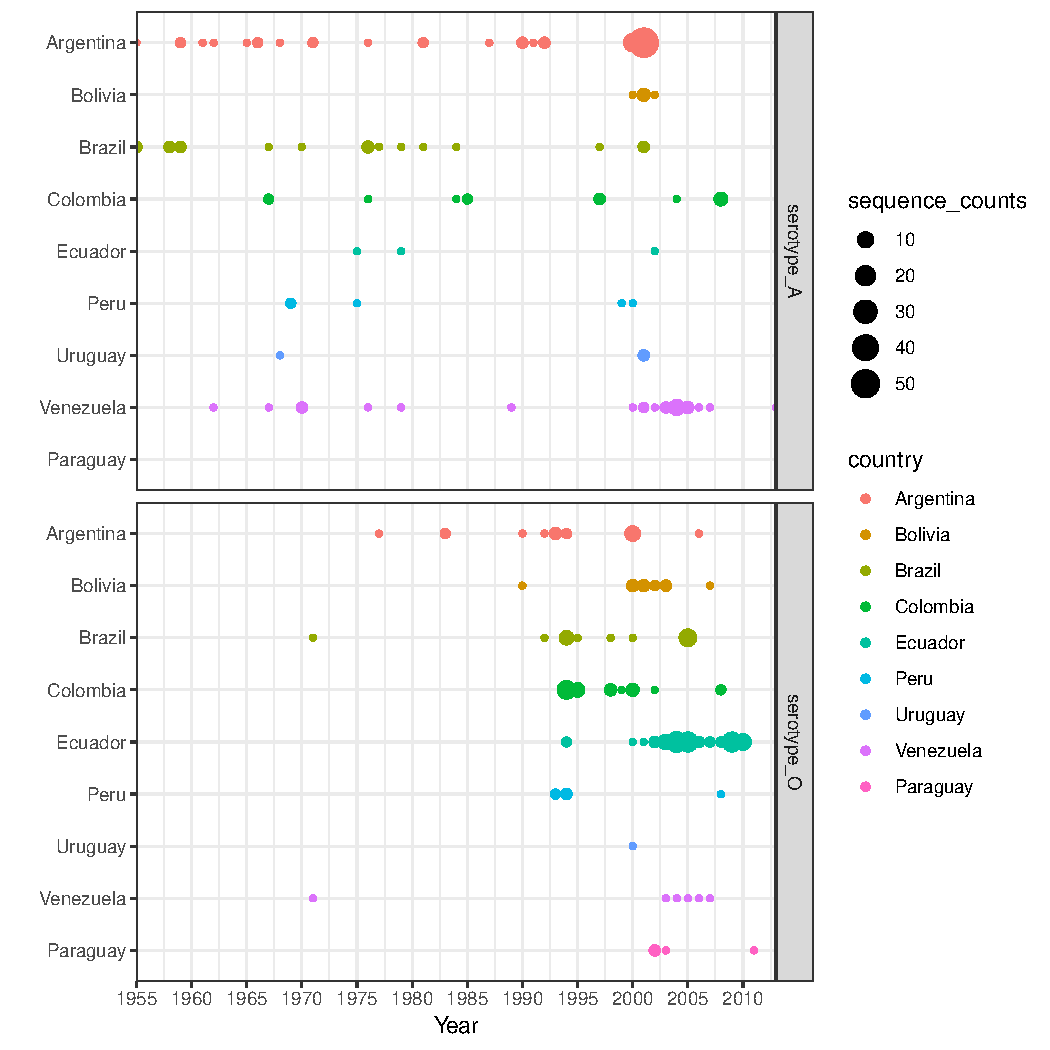
\includegraphics[scale=.80]{FIGURES/PLOTS/sampling_bubble_plot.pdf}
\end{center}
\caption{
\textbf{Spatio-temporal sampling pattern of the sequences used in this study.} Circle radius is proportional to number of sequences.
}
\label{sfig:sampling}
\end{figure}
\end{center}
% %%%%%%%%%%%%%%%%%%
% %%%%%%%%%%%%%%%%%%
\newpage
\begin{center}
\begin{figure}[H]
\begin{center}
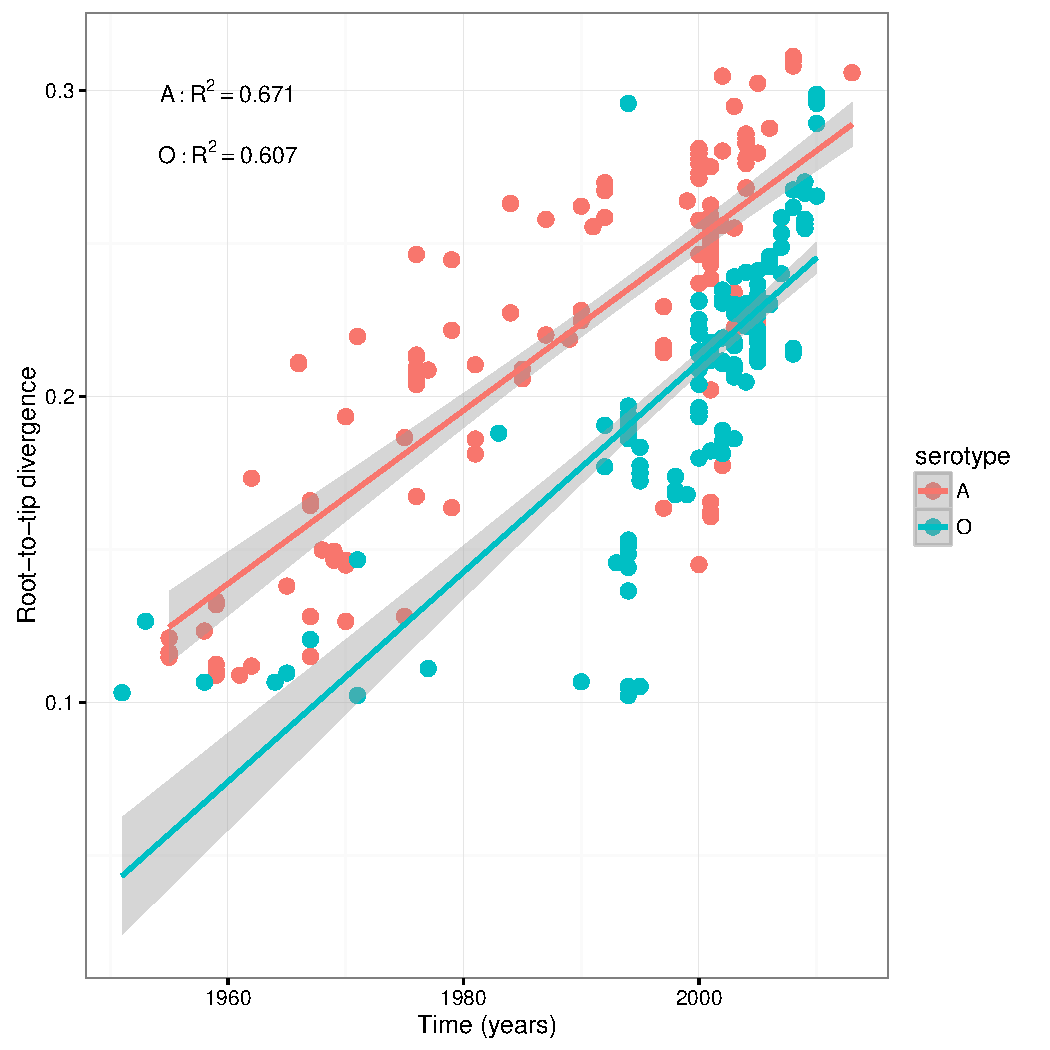
\includegraphics[scale=.75]{FIGURES/PLOTS/rdvs.pdf}
\end{center}
\caption{
\textbf{Root-to-tip divergence against sampling time for serotypes A and O.}
Maximum likelihood phylogenies were constructed with PhyML version 3.0~\cite{M-Guindon2003}. 
We root the trees such that the linear regression between the root-to-tip divergences and sampling times yields the smallest sum of squared residuals using the program Tempest~\citep{M-Rambaut2016}.
The linear trends, along with their 95\% prediction intervals (shaded) are shown.
}
\label{sfig:root-to-tip}
\end{figure}
\end{center}
% %%%%%%%%%%%%%%%%%%
% %%%%%%%%%%%%%%%%%%
\newpage
\begin{center}
\begin{figure}[H]
\begin{center}
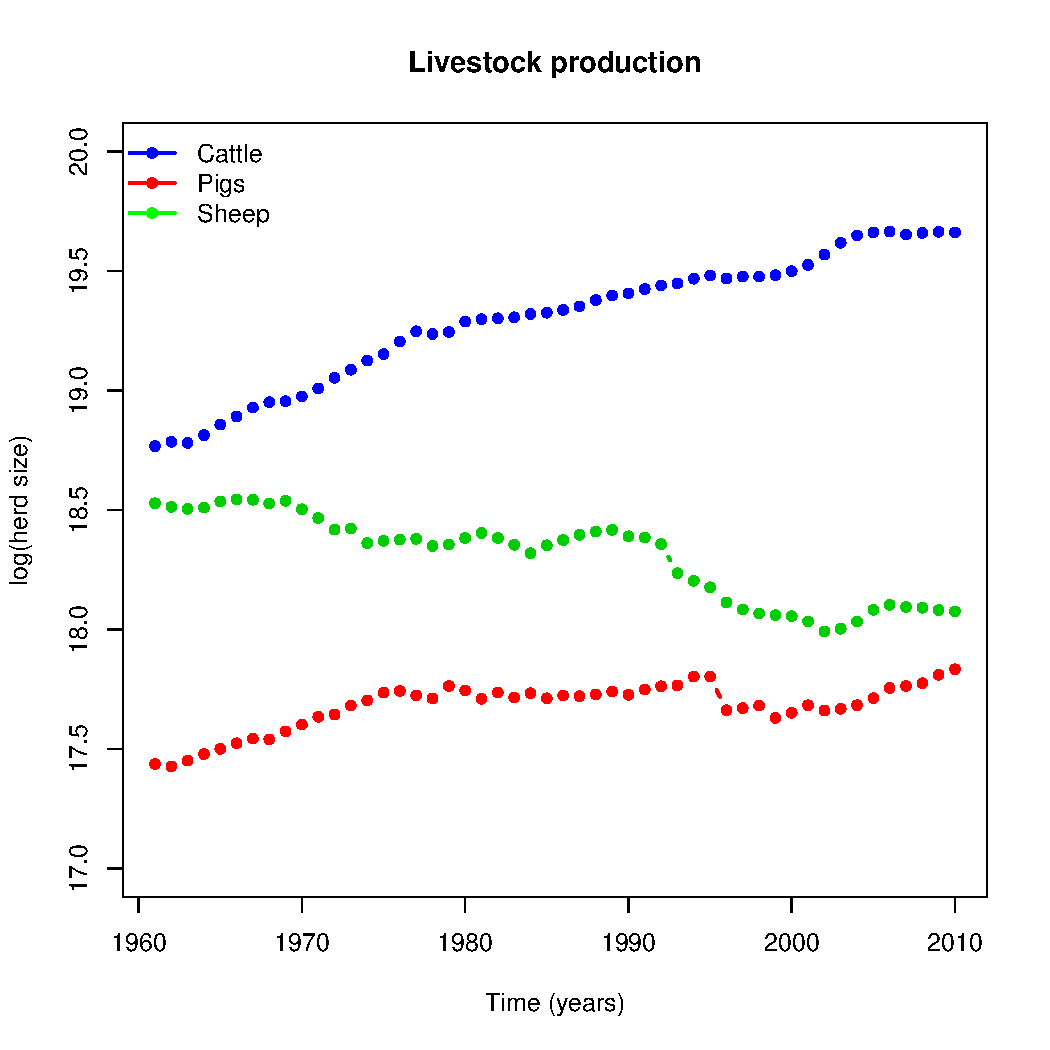
\includegraphics[scale=.80]{FIGURES/PLOTS/production.pdf}
\end{center}
\caption{
\textbf{Production time series for several livestock in South America.}
We show $\log$(\#~of heads) of live animals for pigs, sheep and cattle, goat and horses.
}
\label{sfig:prod}
\end{figure}
\end{center}
% %%%%%%%%%%%%%%%%%%%
% %%%%%%%%%%%%%%%%%%%
\newpage
\begin{center}
\begin{figure}[H]
\begin{center}
\subfigure[]{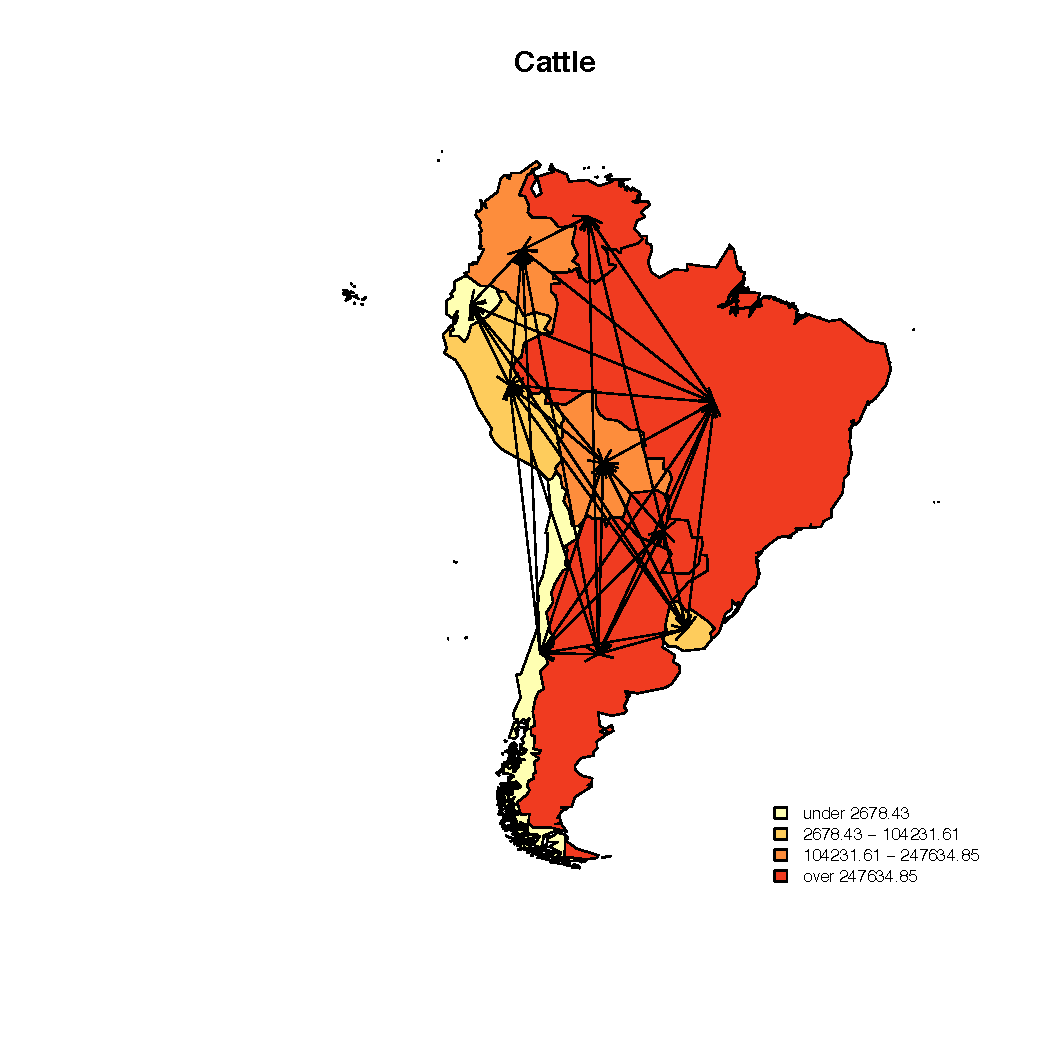
\includegraphics[scale=.400]{FIGURES/PLOTS/tradenets_cattle_s=0.pdf}}
\subfigure[]{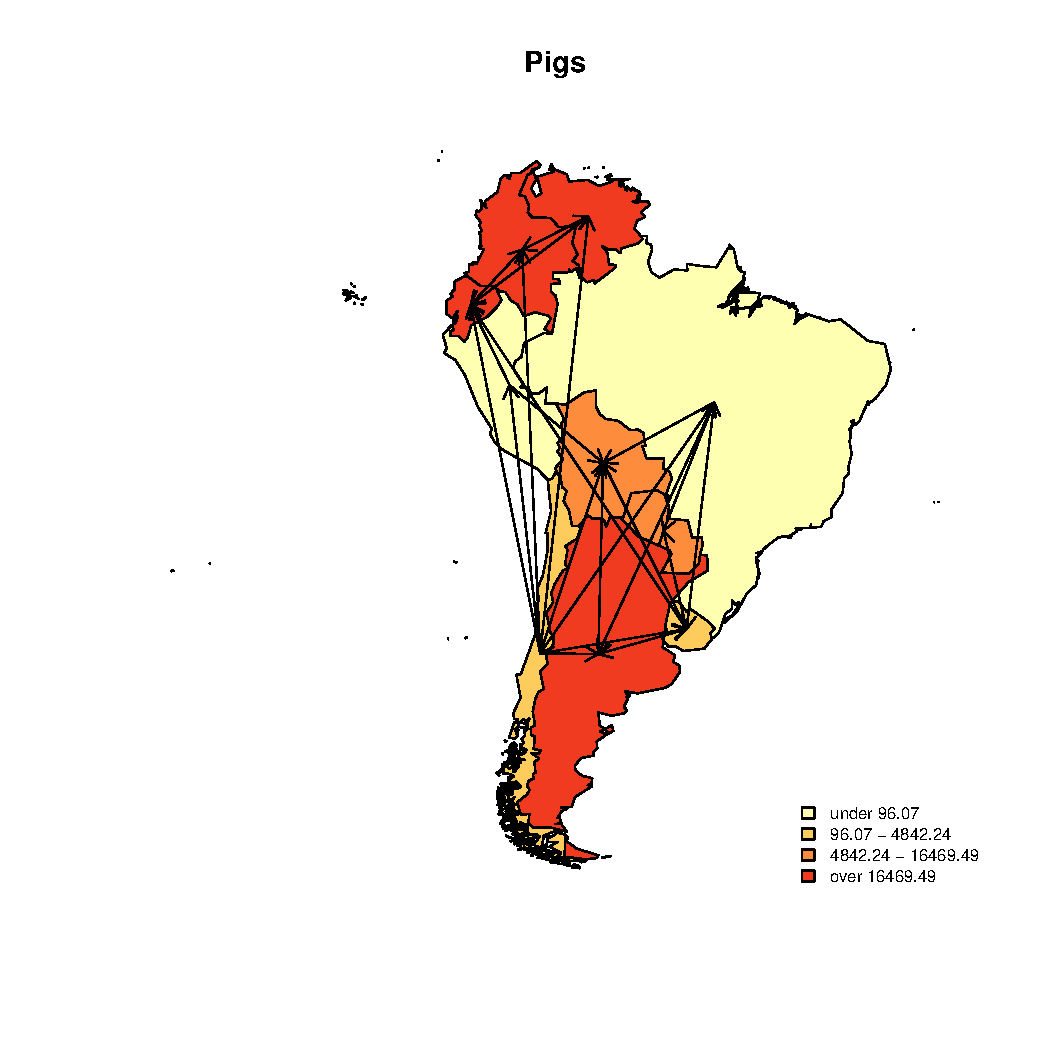
\includegraphics[scale=.400]{FIGURES/PLOTS/tradenets_pig_s=0.pdf}} \\
\subfigure[]{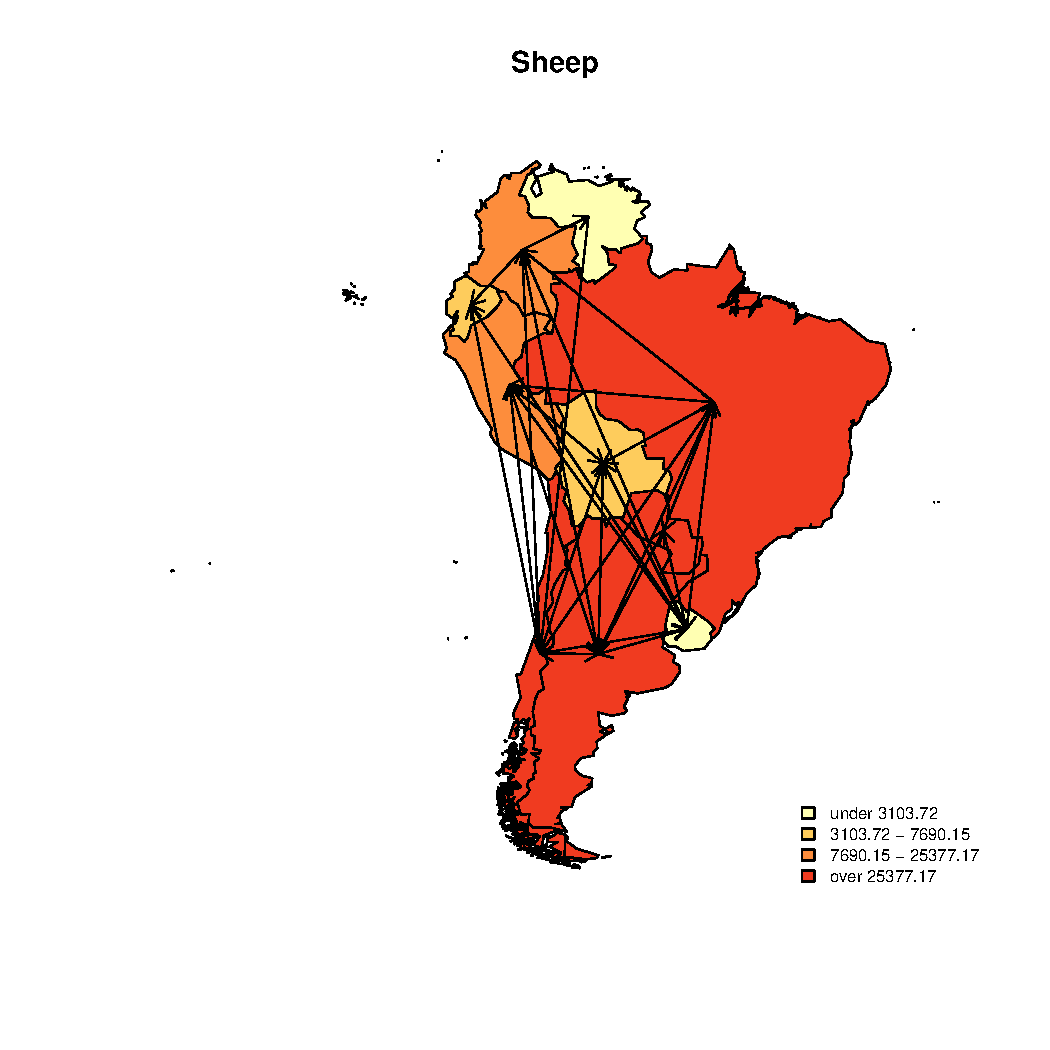
\includegraphics[scale=.400]{FIGURES/PLOTS/tradenets_sheep_s=0.pdf}}
\end{center}
\caption{
\textbf{Spatial networks of livestock trade in South America.}
We represent the total trade of live animals from $1986$ to $2017$.
Arrows connect countries if there was a non-zero number of exchanges between them.
Colour scale represents total exports in number of live animals.
In agreement with the data presented in Figure~\ref{sfig:prod}, the cattle network is the most connected, indicating that not only the number of animals has increased, but also the migration of this particular host is more frequent. 
Note the long range trade routes of sheep between Argentina and Colombia, which are absent from the pig network.
}
\label{sfig:tradenets}
\end{figure}
\end{center}
% %%%%%%%%%%%%%%%%%%%
% %%%%%%%%%%%%%%%%%%%
\newpage
\begin{center}
\begin{figure}[H]
\begin{center}
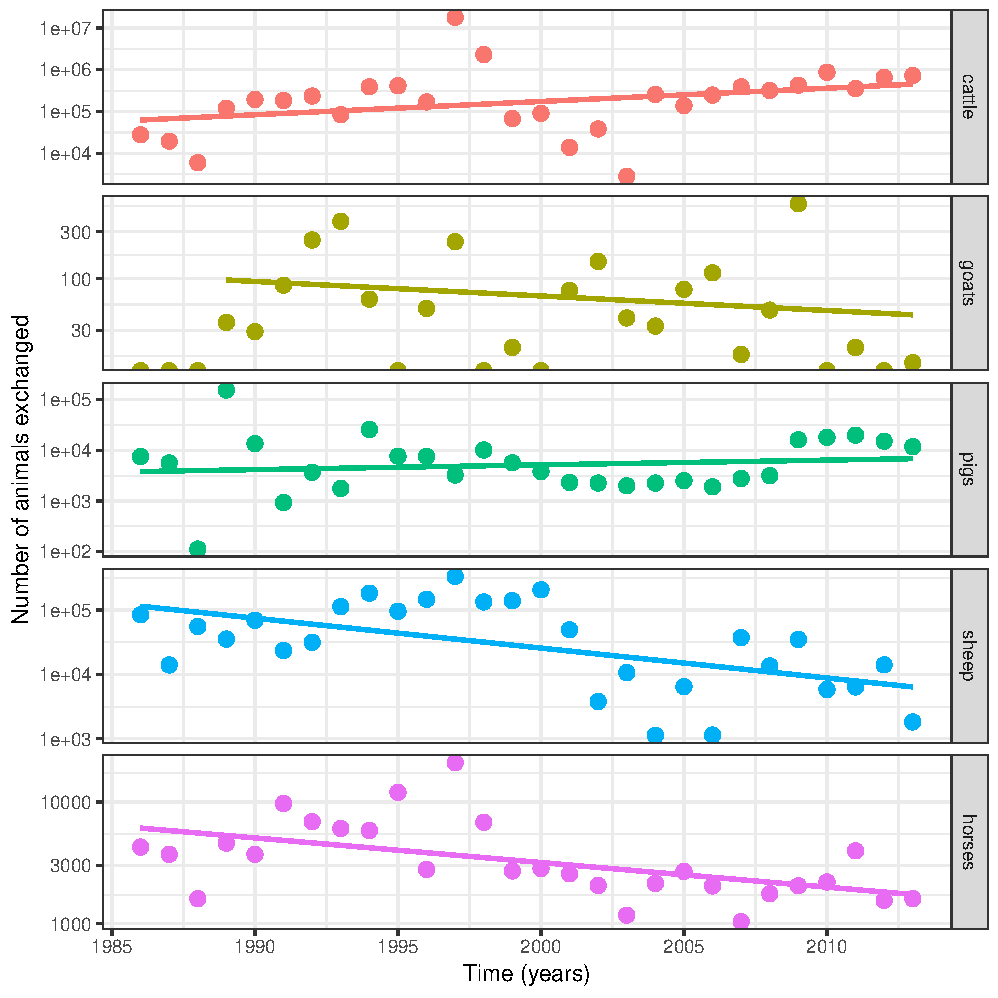
\includegraphics[scale=.80]{FIGURES/PLOTS/trade_through_time.pdf}
\end{center}
\caption{
\textbf{Overall livestock trade in South America through time.}
We show $\log$(\#~of heads) of live animals traded for pigs, sheep and cattle, goat and horses.
Solid lines are linear trends fitted using ordinary least squares.
}
\label{sfig:trade_temporal}
\end{figure}
\end{center}
% %%%%%%%%%%%%%%%%%%%
% %%%%%%%%%%%%%%%%%%%
\newpage
\begin{center}
\begin{figure}[H]
\begin{center}
\subfigure[]{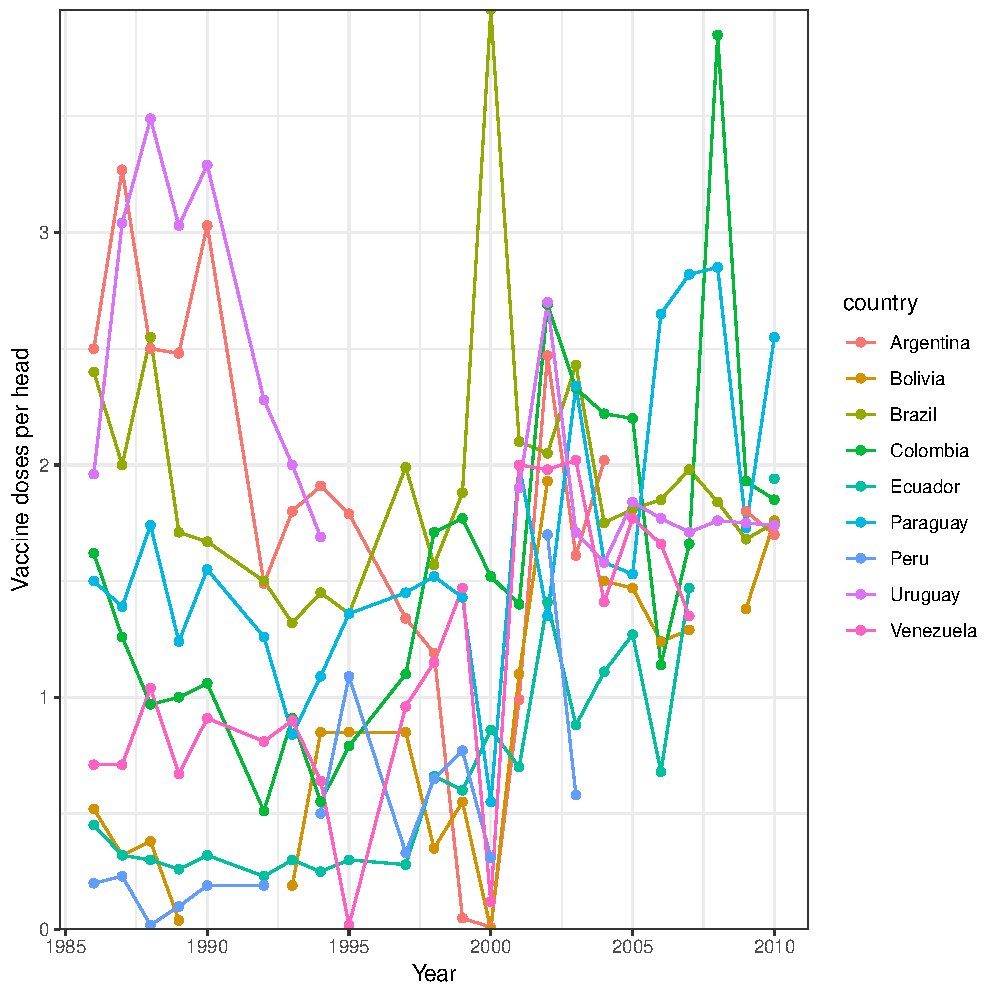
\includegraphics[scale=.600]{FIGURES/PLOTS/vaccination_per_country_time.pdf}} \\
\subfigure[]{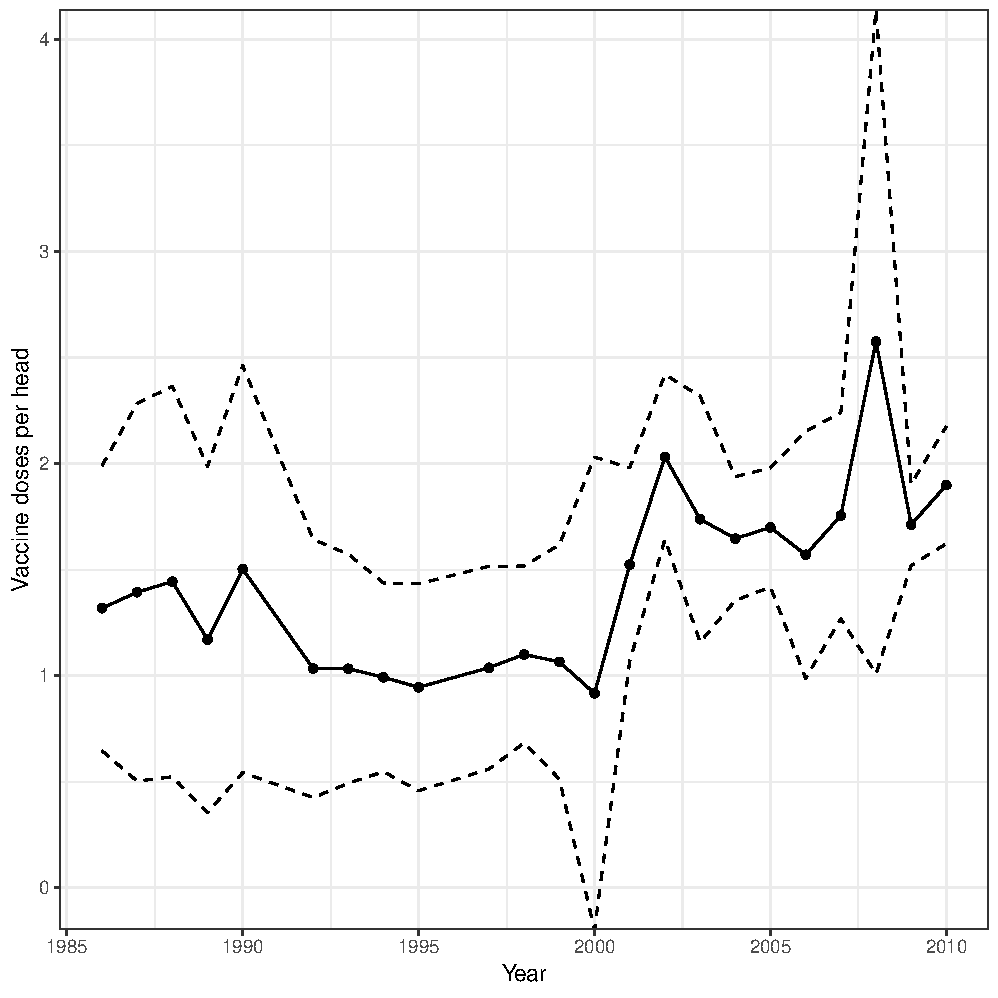
\includegraphics[scale=.600]{FIGURES/PLOTS/vaccination_overall_time.pdf}}
\end{center}
\caption{
\textbf{FMD vaccination in South America through time.}
We show the number of vaccine doses per cattle head per country (Panel a) and overall (Panel b).
In panel b the solid line shows the average and the dashed lines show Student t empirical intervals (see text).
}
\label{sfig:vaccination_temporal}
\end{figure}
\end{center}
% %%%%%%%%%%%%%%%%
% %%%%%%%%%%%%%%%%
% %%%%%%%%%%%%%%%%%%%
% %%%%%%%%%%%%%%%%%%%
\newpage
\begin{center}
\begin{figure}[H]
\begin{center}
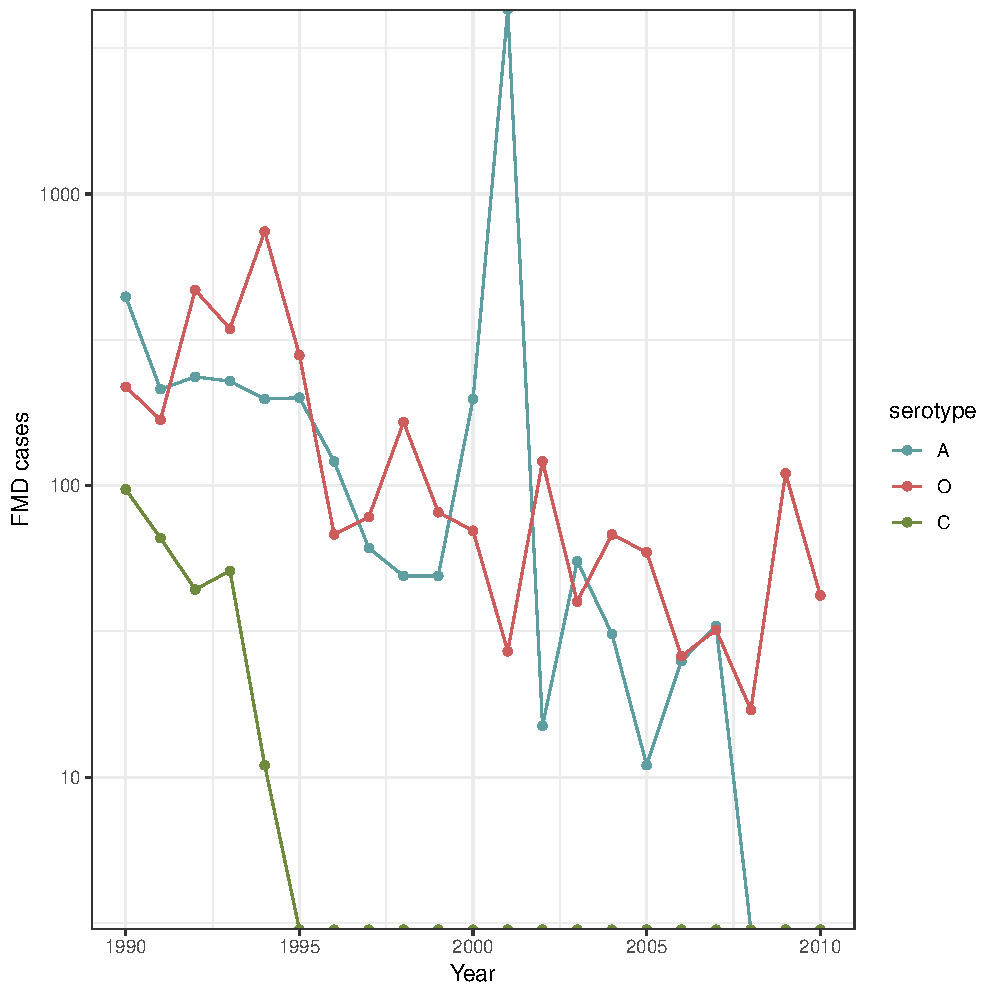
\includegraphics[scale=.600]{FIGURES/PLOTS/cases_per_serotype_per_time.pdf}
\end{center}
\caption{
\textbf{FMD cases per serotype in South America through time.}
We show the number of reported FMD cases per serotype.
}
\label{sfig:case_temporal}
\end{figure}
\end{center}
% %%%%%%%%%%%%%%%%
% %%%%%%%%%%%%%%%%
% \newpage
\begin{center}
\begin{figure}[H]
\begin{center}
\subfigure[]{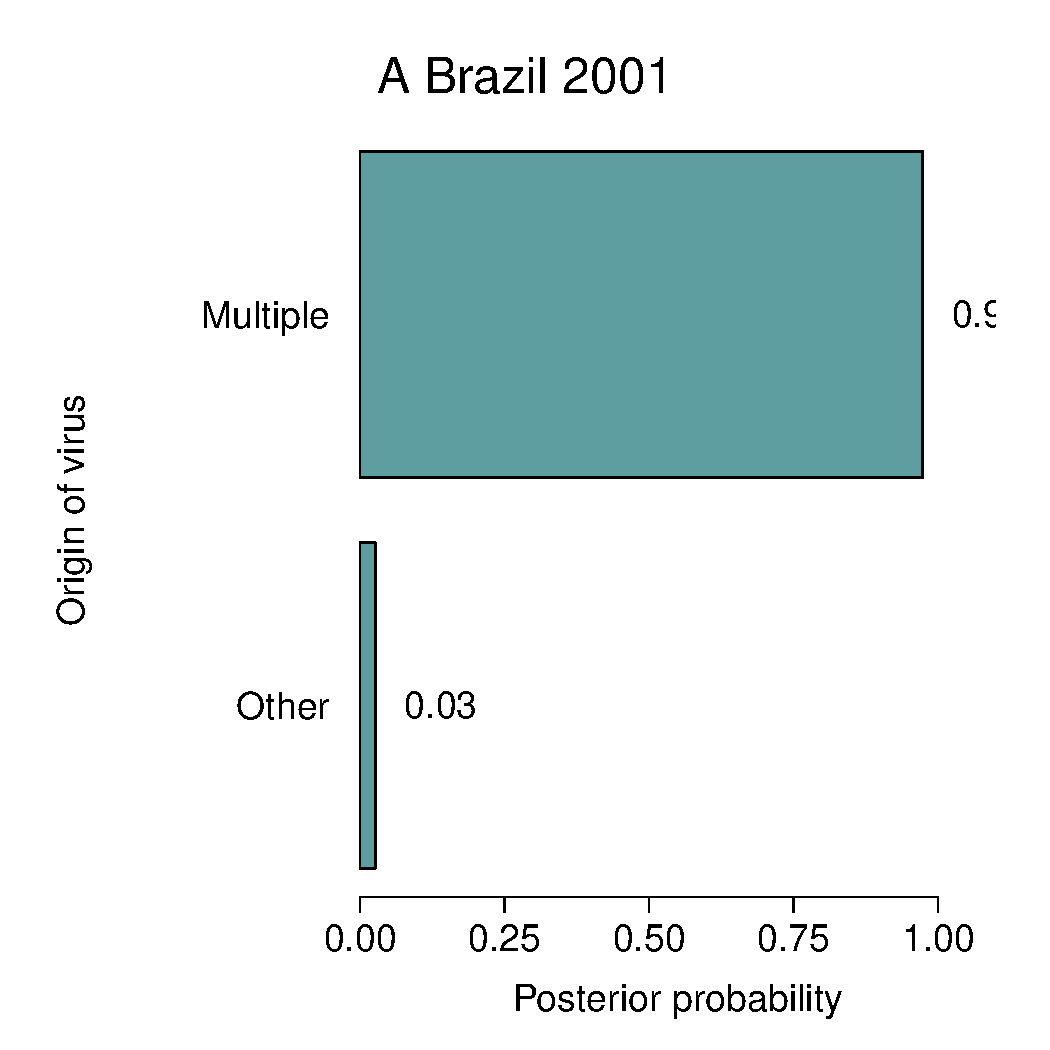
\includegraphics[scale=.40]{FIGURES/PLOTS/Origins_A_Brazil_2001.pdf}}
\subfigure[]{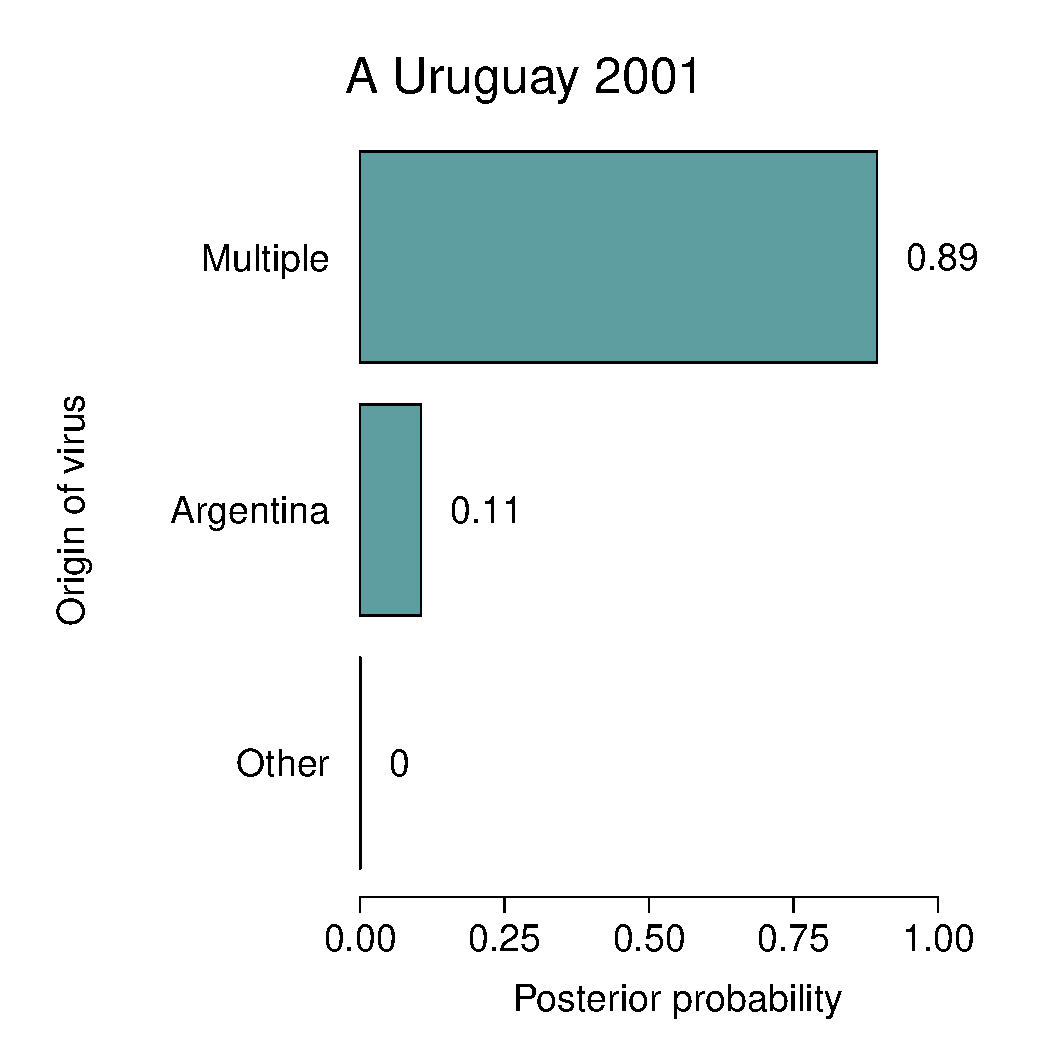
\includegraphics[scale=.40]{FIGURES/PLOTS/Origins_A_Uruguay_2001.pdf}}\\
\subfigure[]{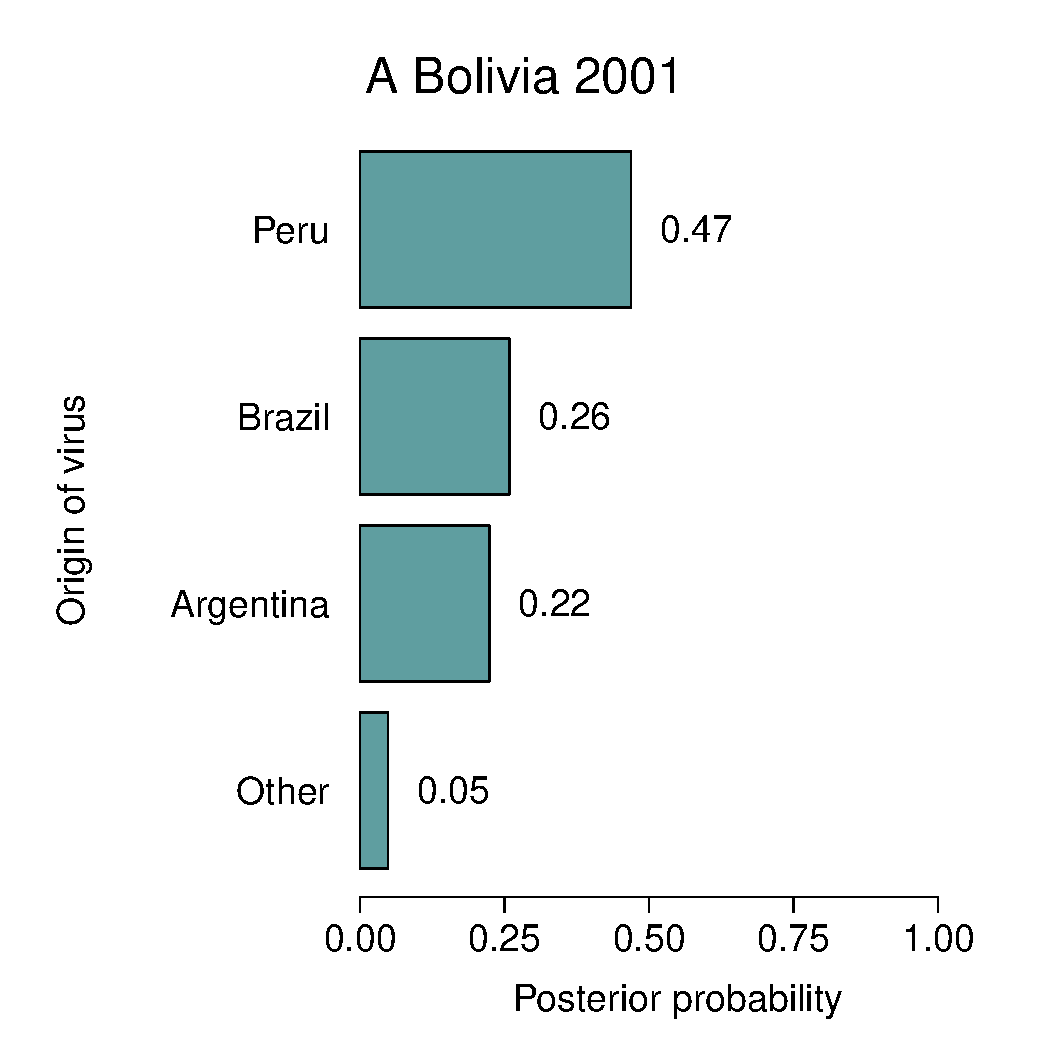
\includegraphics[scale=.40]{FIGURES/PLOTS/Origins_A_Bolivia_2001.pdf}}
\subfigure[]{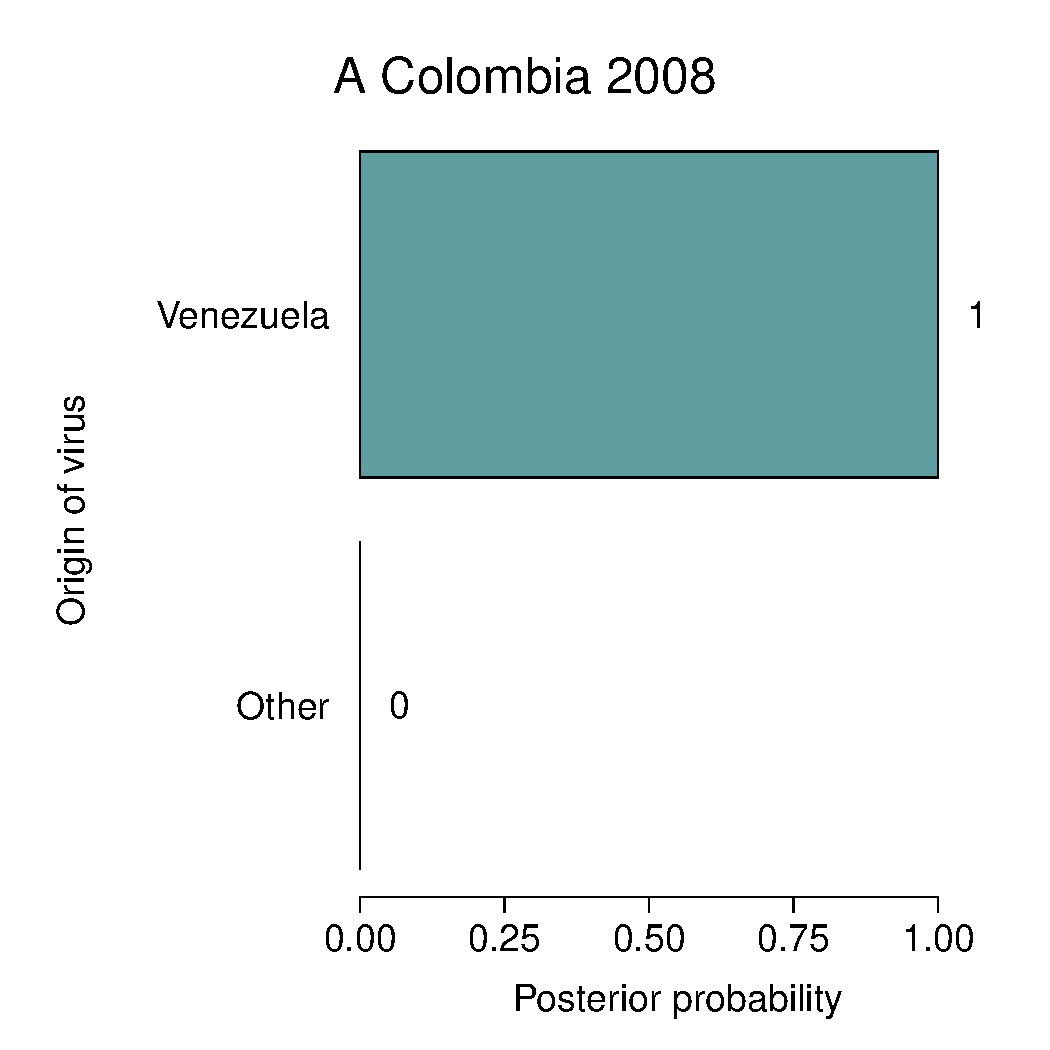
\includegraphics[scale=.40]{FIGURES/PLOTS/Origins_A_Colombia_2008.pdf}}\\
\subfigure[]{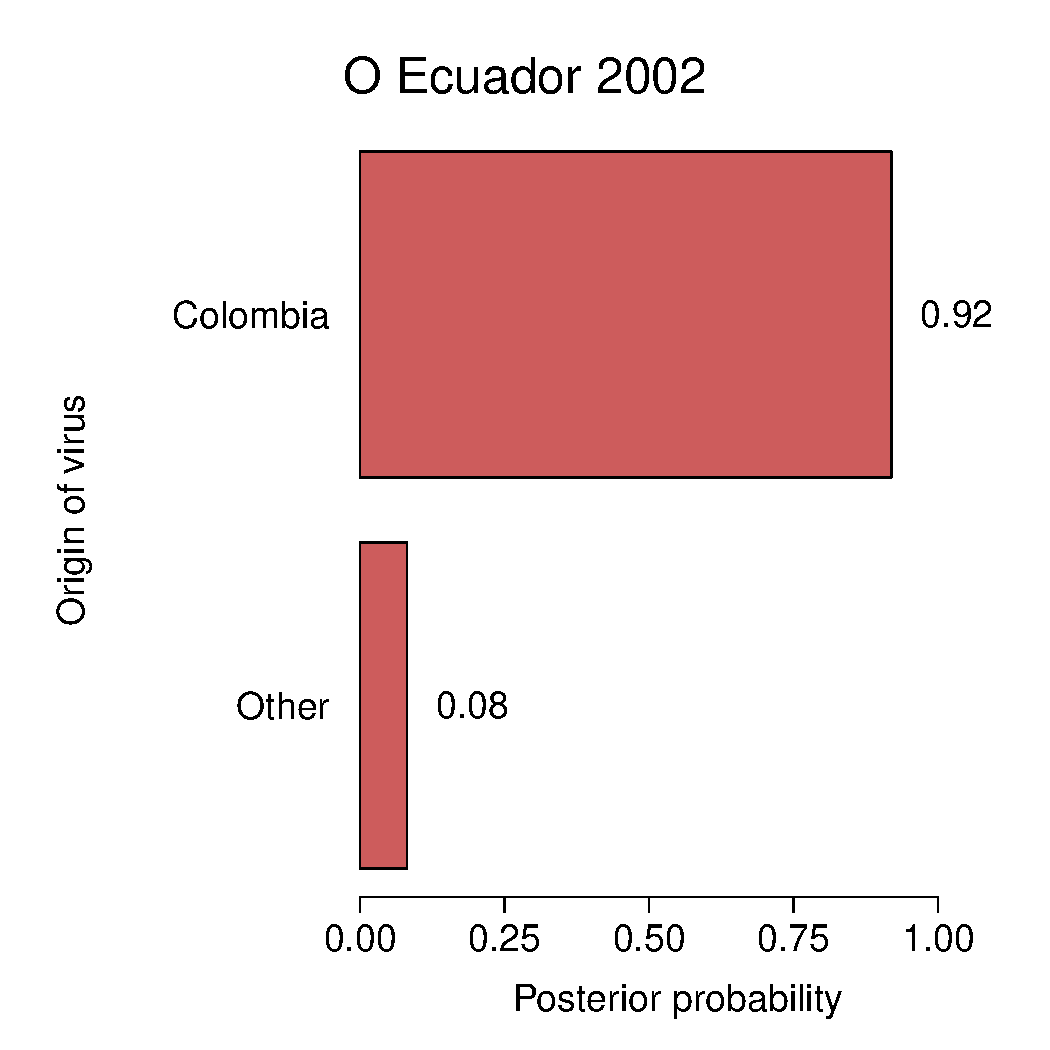
\includegraphics[scale=.40]{FIGURES/PLOTS/Origins_O_Ecuador_2002.pdf}}
\subfigure[]{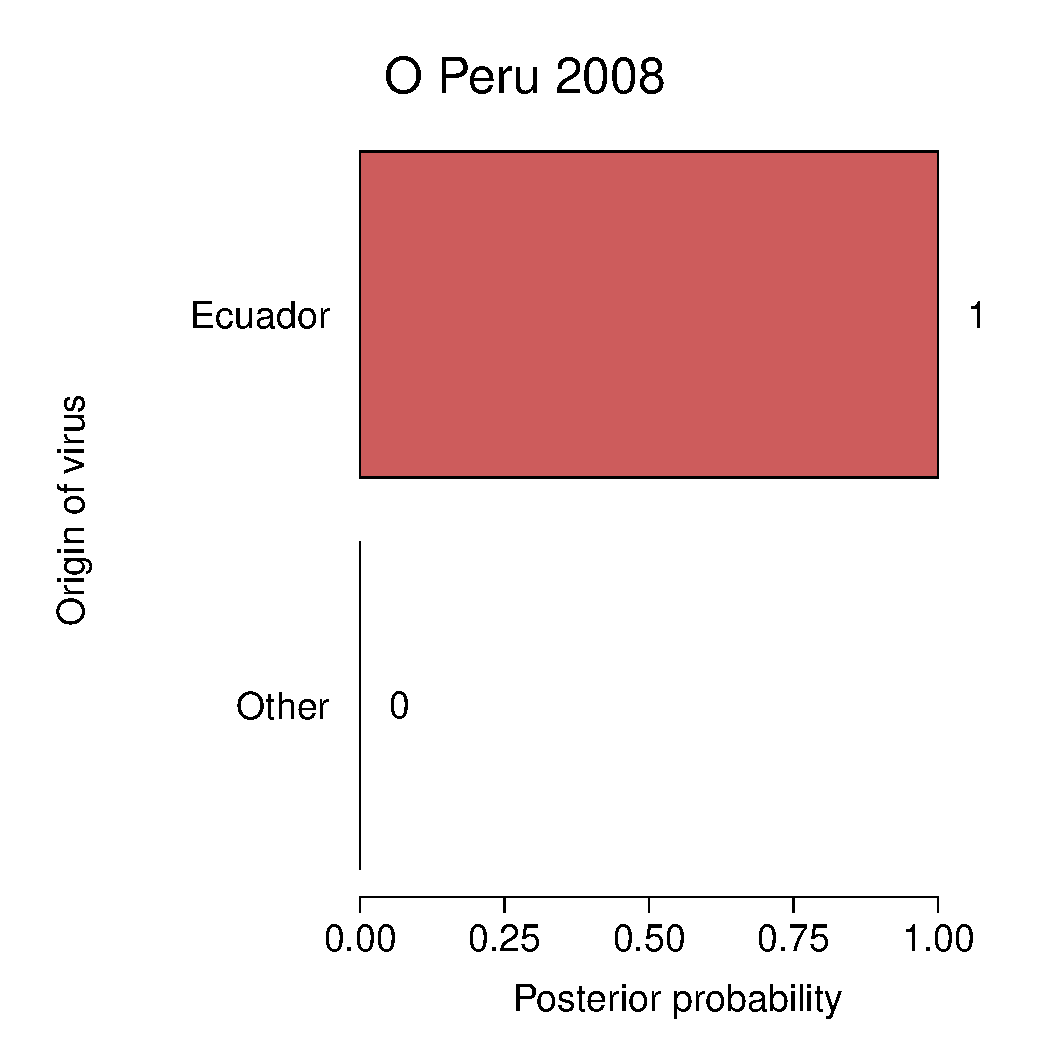
\includegraphics[scale=.40]{FIGURES/PLOTS/Origins_O_Peru_2008.pdf}}
\end{center}
\caption{\textbf{Epidemic tracing of FMDV in South America -- extra results}.
}
\label{sfig:epitrac}
\end{figure}
\end{center}
% %%%%%%%%%%%%%%%%%%%
% %%%%%%%%%%%%%%%%%%%
% \newpage
% \begin{figure}[H]
% \begin{center}
% \subfigure[]{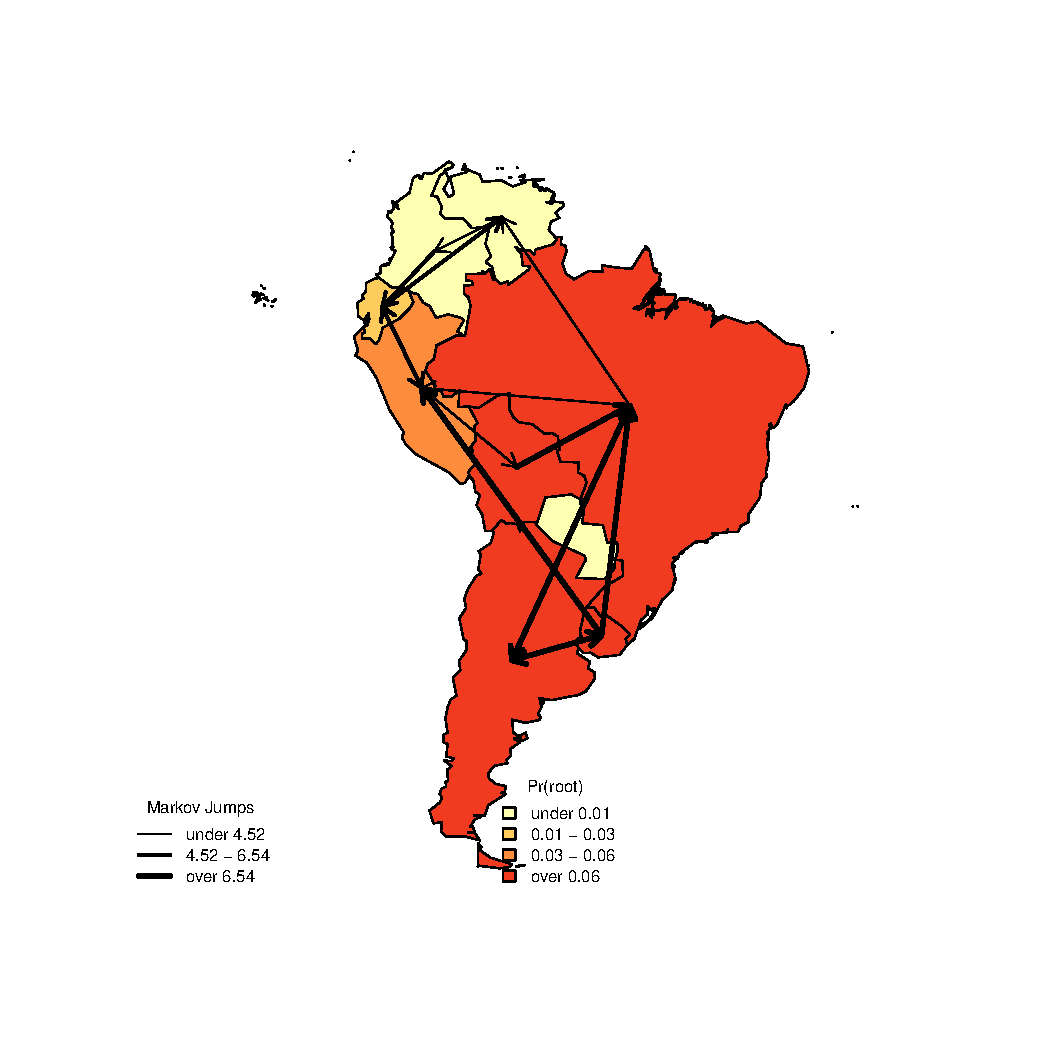
\includegraphics[scale=.350]{FIGURES/A_ss1.pdf}}
% \subfigure[]{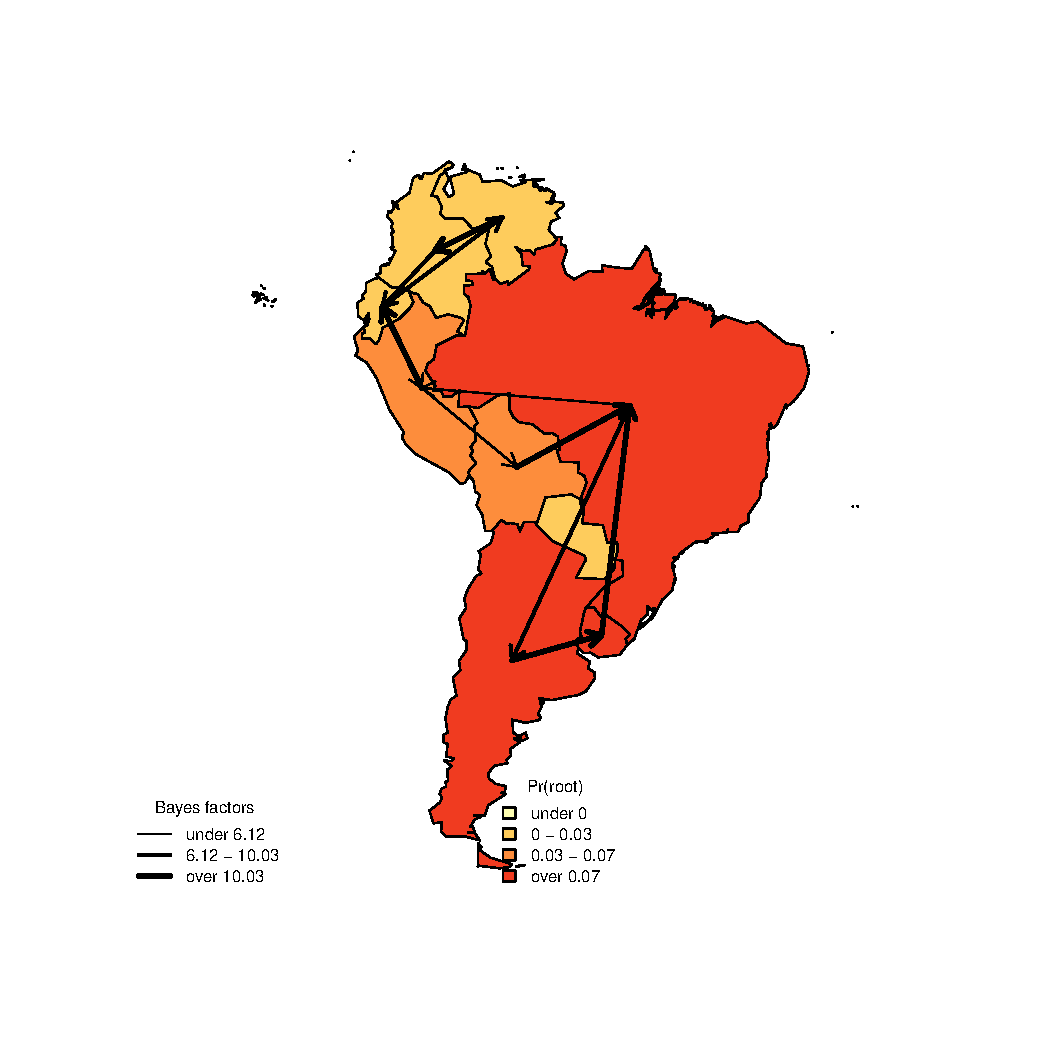
\includegraphics[scale=.350]{FIGURES/A_ss2.pdf}}\\
% \subfigure[]{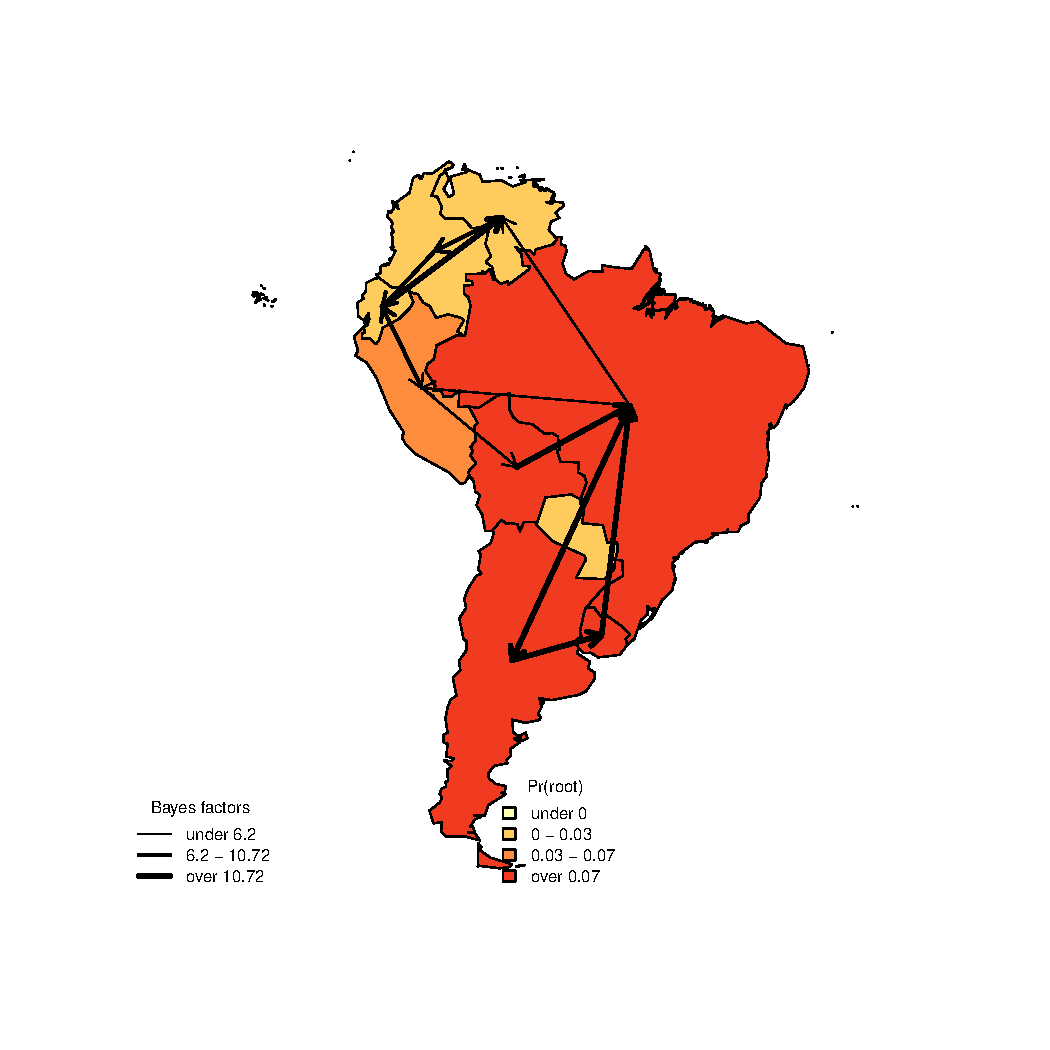
\includegraphics[scale=.350]{FIGURES/A_ss3.pdf}}
% \subfigure[]{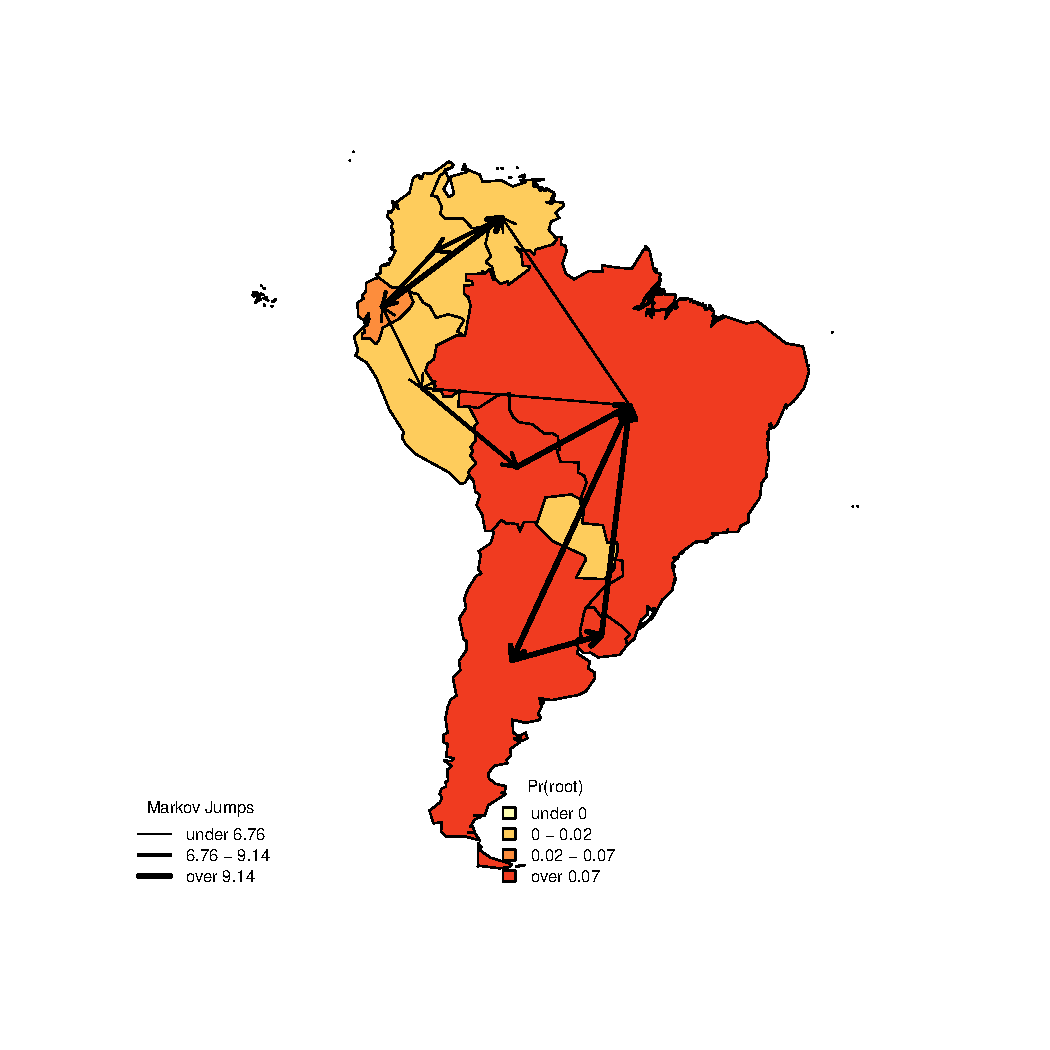
\includegraphics[scale=.350]{FIGURES/A_ss4.pdf}}\\
% \subfigure[]{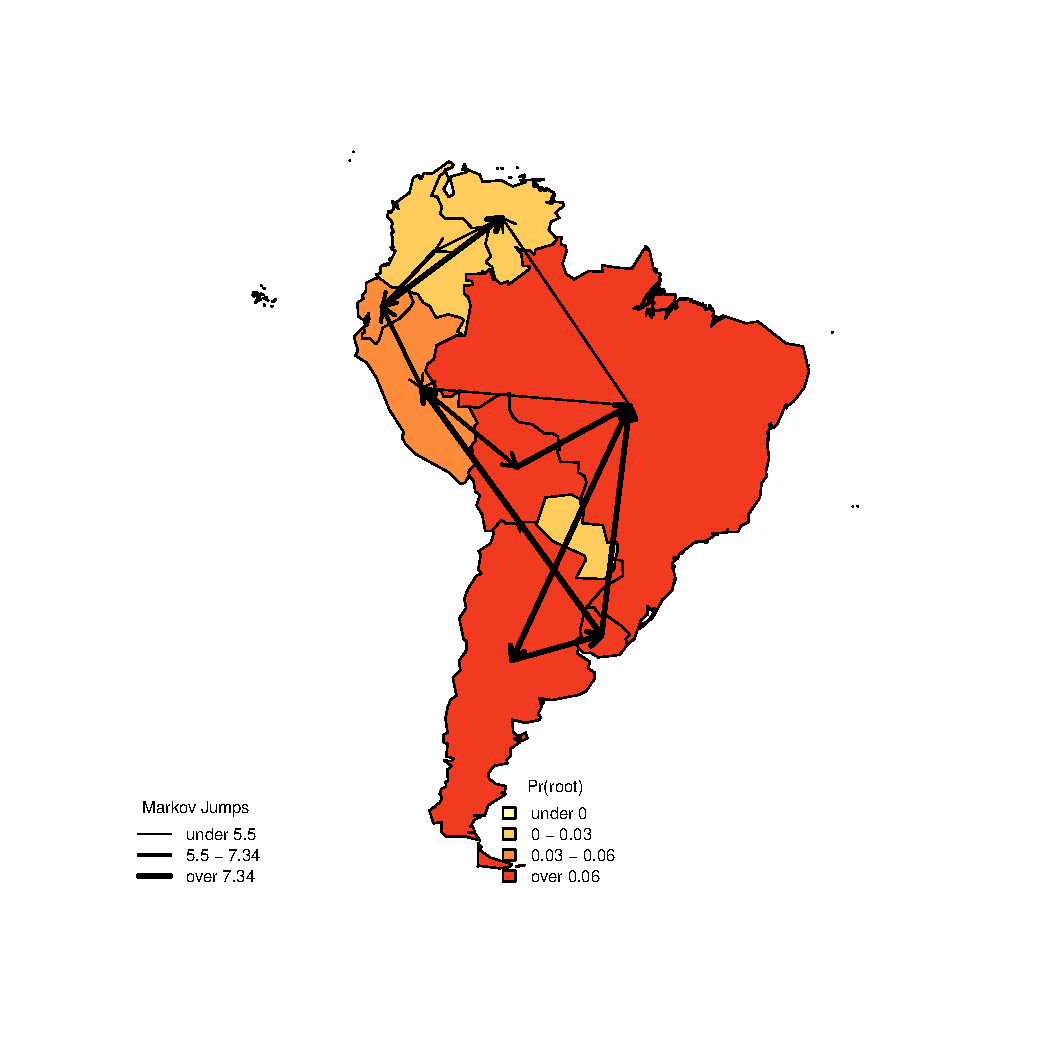
\includegraphics[scale=.350]{FIGURES/A_ss5.pdf}}
% \caption{}
% \label{sfig:bssvsA}
% \end{center}
% \end{figure}
% %%%%%%%%%%%%%%%
% %%%%%%%%%%%%%%%
% \newpage
% \begin{figure}[H]
% \begin{center}
% \subfigure[]{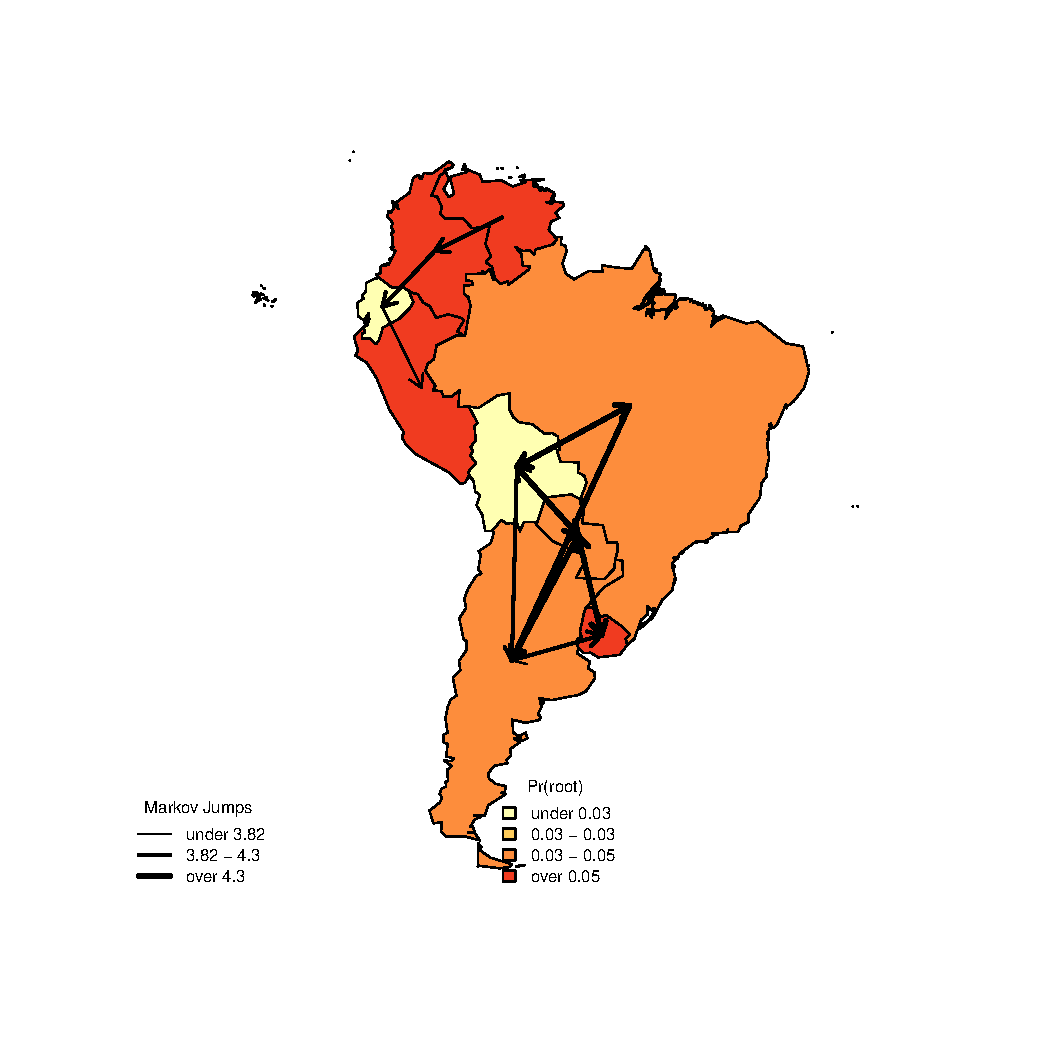
\includegraphics[scale=.350]{FIGURES/O_ss1.pdf}}
% \subfigure[]{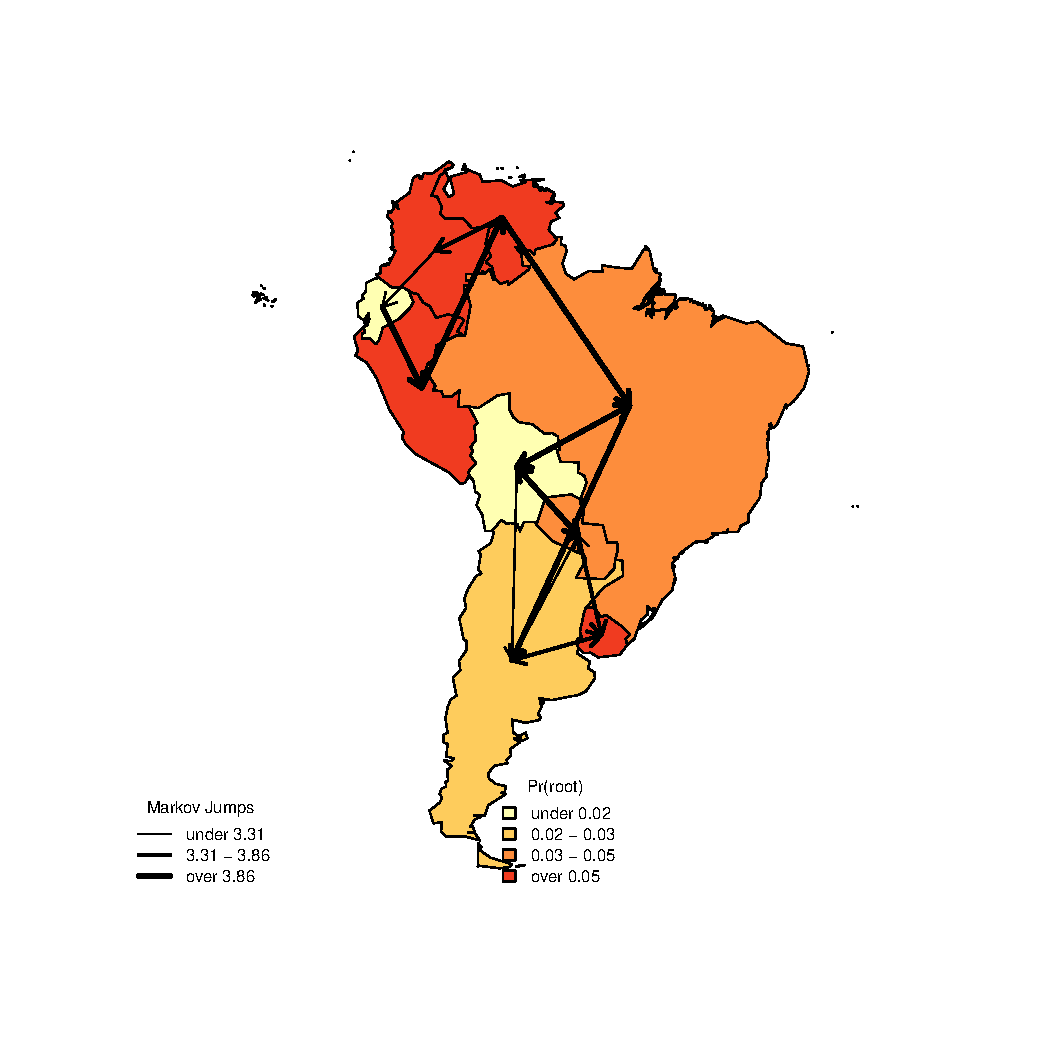
\includegraphics[scale=.350]{FIGURES/O_ss2.pdf}}\\
% \subfigure[]{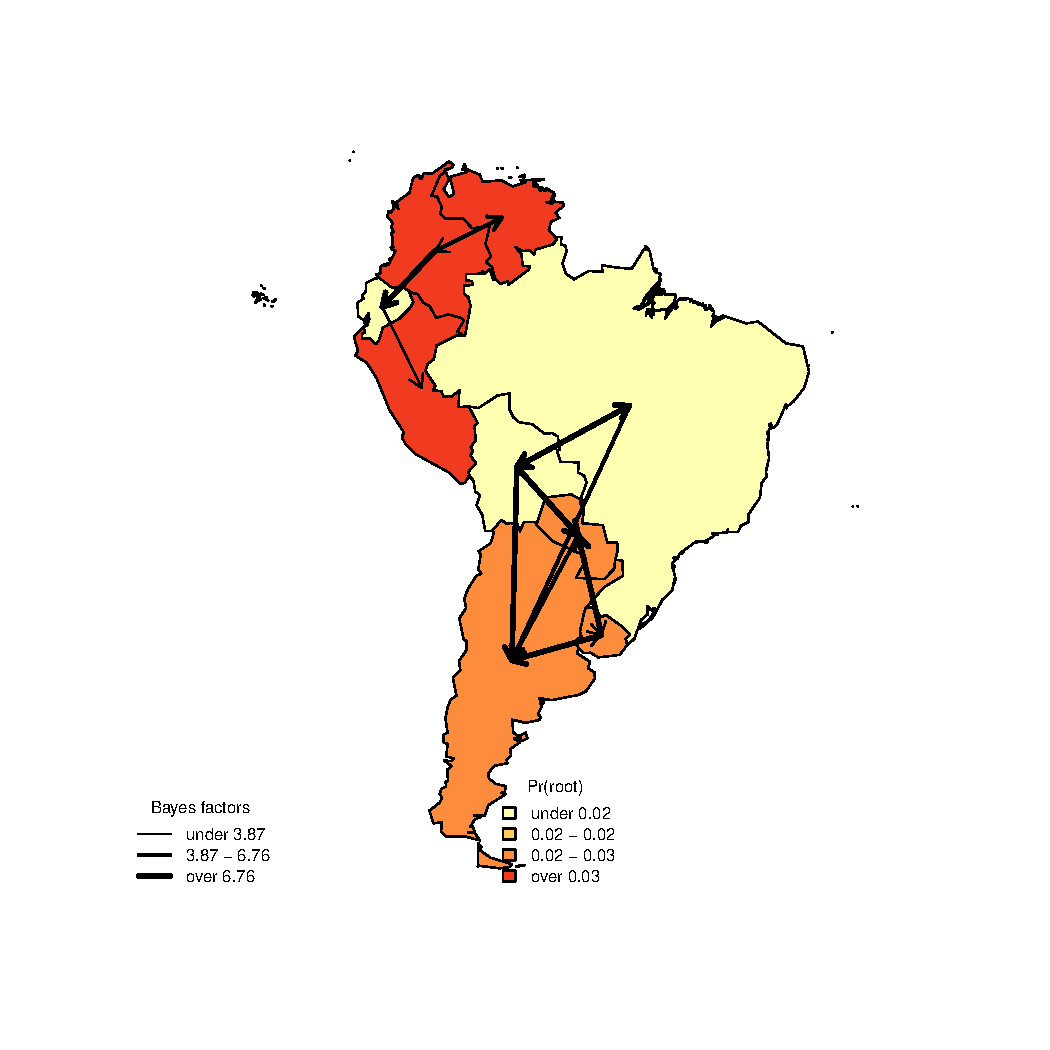
\includegraphics[scale=.350]{FIGURES/O_ss3.pdf}}
% \subfigure[]{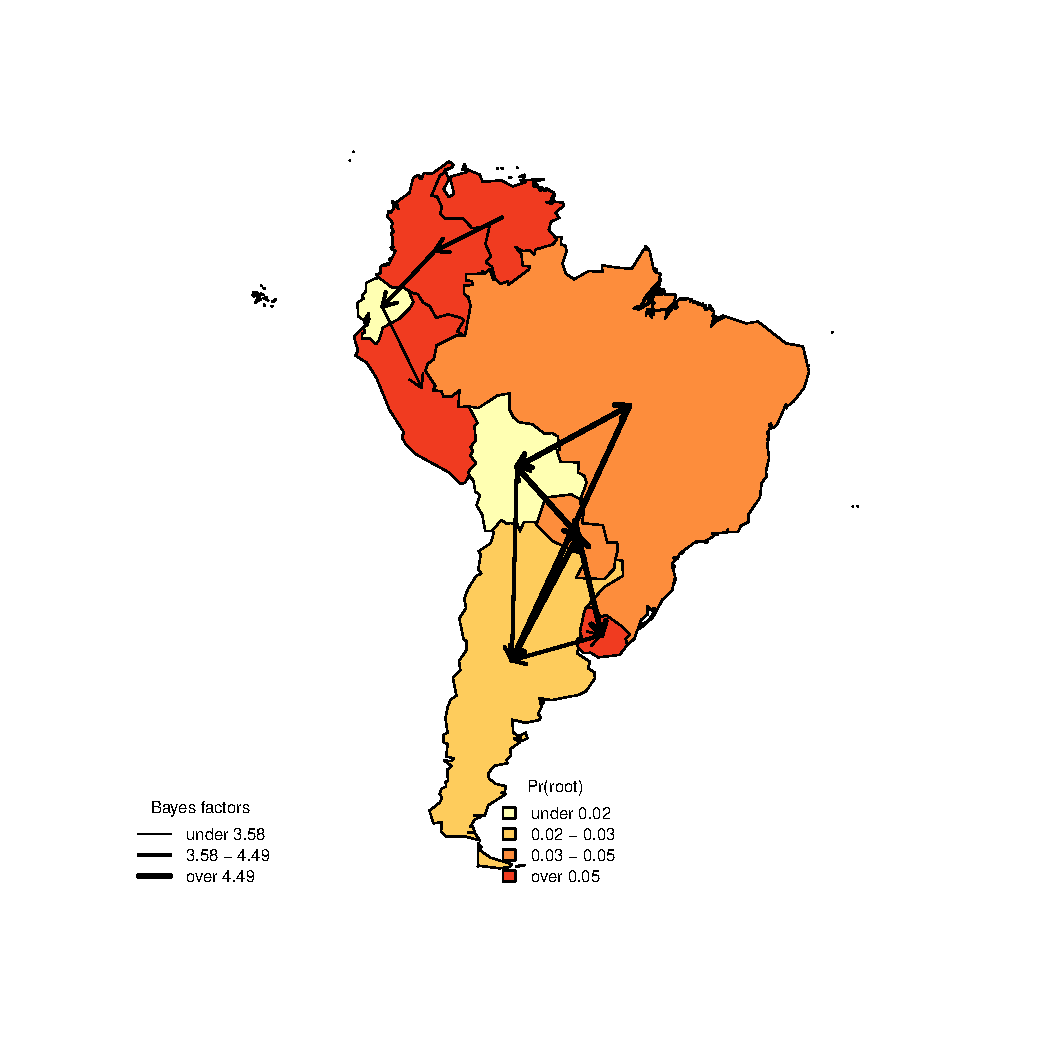
\includegraphics[scale=.350]{FIGURES/O_ss4.pdf}}\\
% \subfigure[]{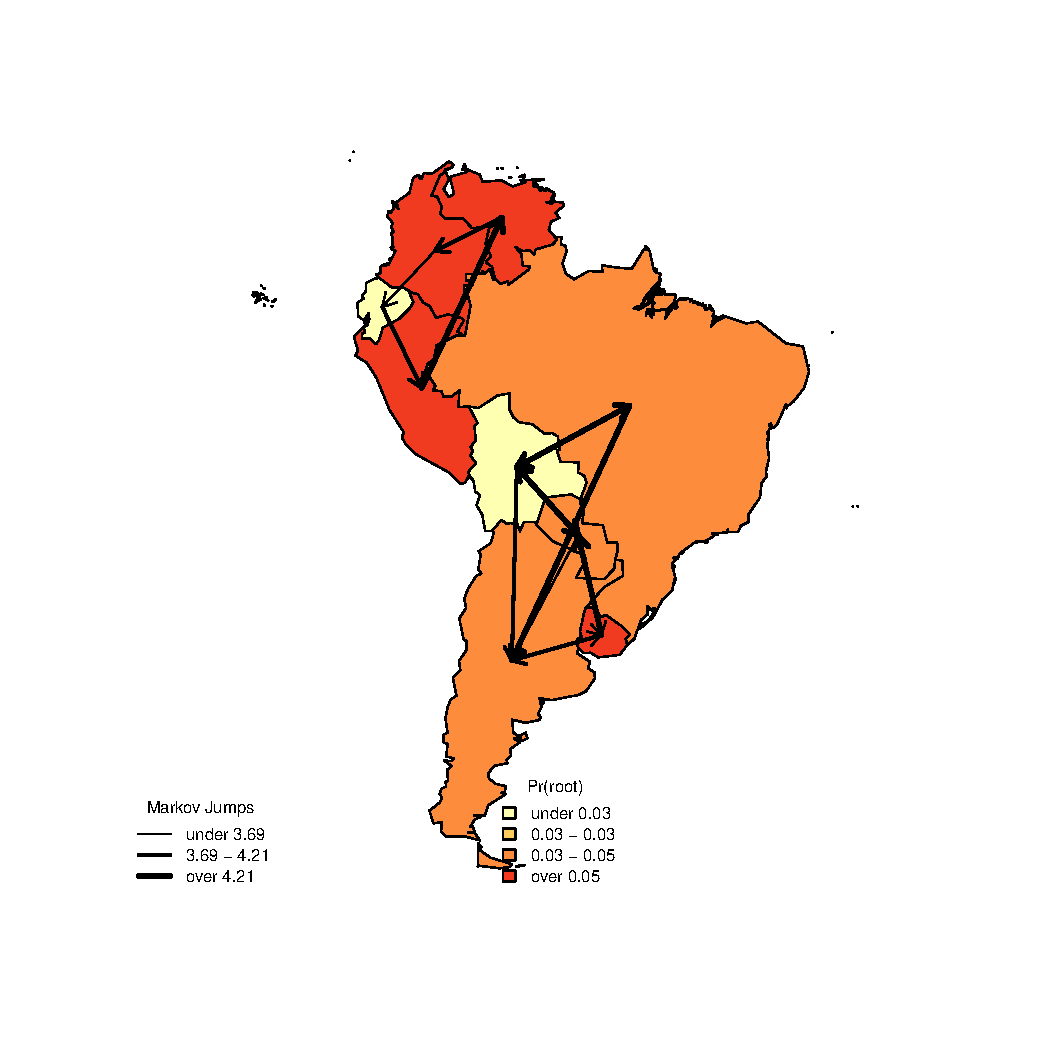
\includegraphics[scale=.350]{FIGURES/O_ss5.pdf}}
% \end{center}
% \caption{}
% \label{sfig:bssvsO}
% \end{figure}
% %%%%%%%%%%%%%%%%
% %%%%%%%%%%%%%%%%
% \newpage
% \begin{figure}[H]
% \begin{center}
% \subfigure[]{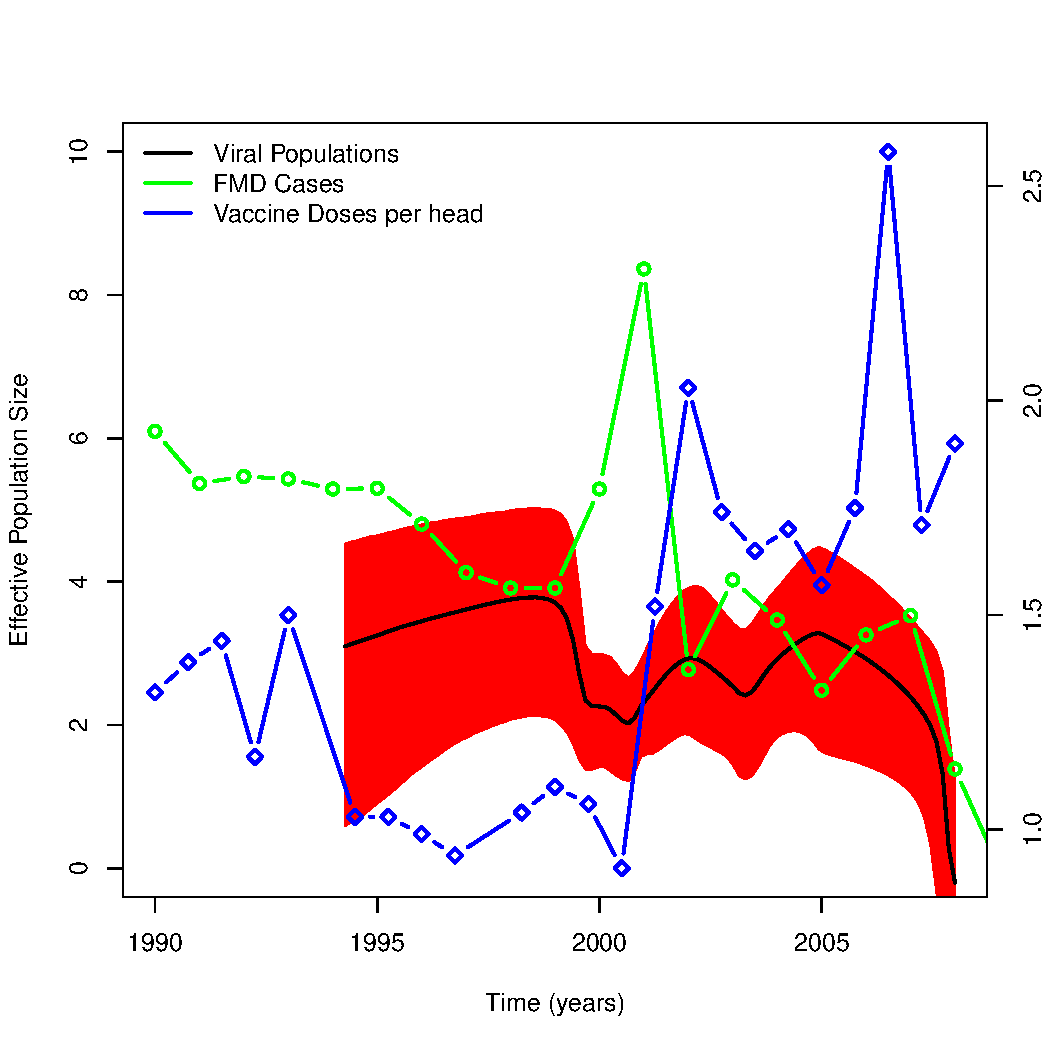
\includegraphics[scale=.60]{FIGURES/SFig_A2000sky.pdf}}\\
% \subfigure[]{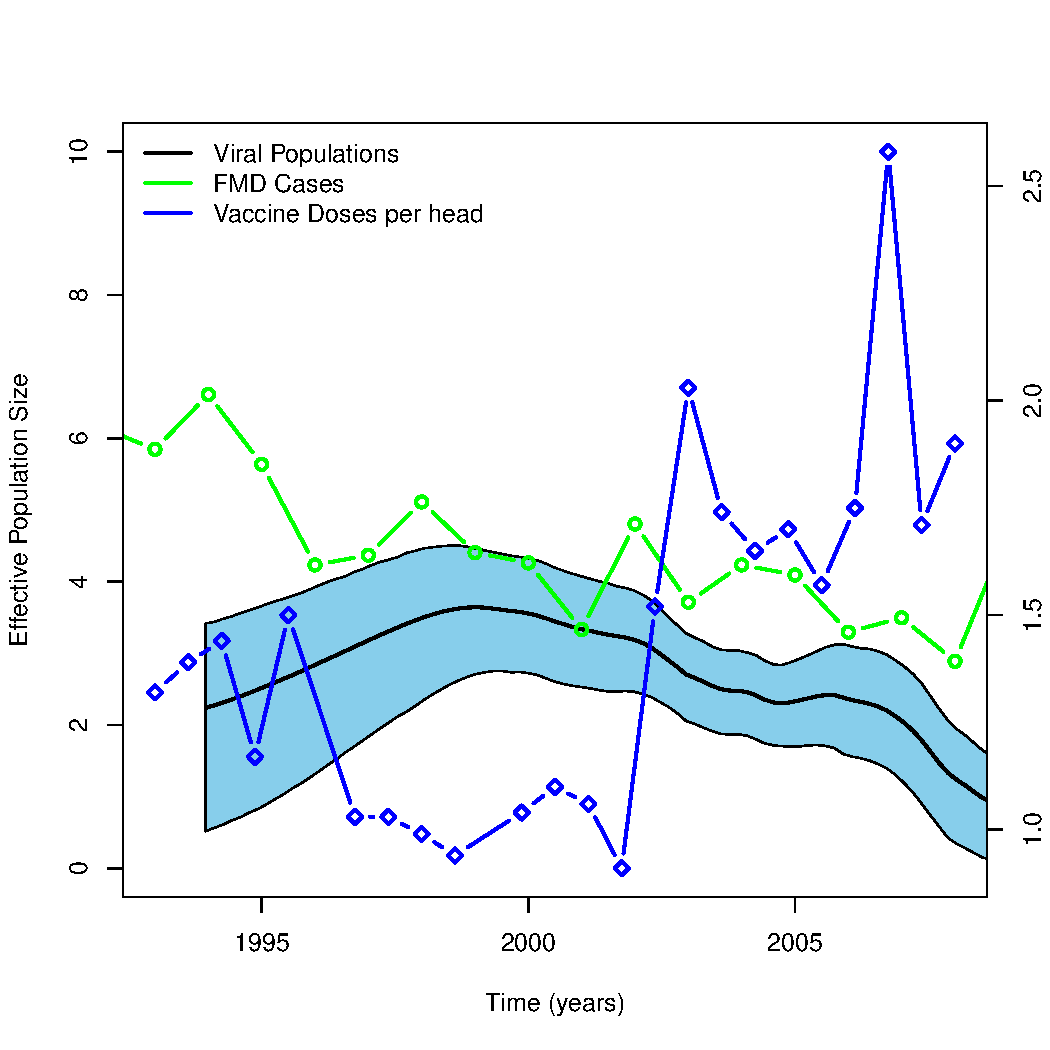
\includegraphics[scale=.60]{FIGURES/SFig_O2000sky.pdf}}
% \end{center}
% \caption{}
% \label{sfig:only2000sky}
% \end{figure}
% %%%%%%%%%%%%%%%%
% %%%%%%%%%%%%%%%%
% \newpage
% \begin{table}[H]
% \caption{\textbf{Model selection using path sampling (PS) and stepping-stone sampling (SS) to determine the tree prior (coalescent) model and clock for both serotypes.}
% UCLD = uncorrelated relaxed clock with an underlying log-normal distribution; UCED = uncorrelated relaxed clock with an underlying exponential distribution.
% Best fitting models (highest log marginal likelihood obtained using SS) are highlighted in bold.
% The more flexible non-parametric skyride tree prior clearly outperforms the assumption of a constant population size, which is consistent with the fact that FMDV (both serotypes) has experienced periods of population expansion, i.e. transmission within the time frame considered.
% The assumption of a single rate for every lineage in the phylogeny was also rejected for both serotypes.
% Remarkably, the best fitting relaxed clock models are different for each serotype, suggesting different branch (lineage) level heterogeneity between serotypes.
% }
% \begin{center}
% \begin{tabular}{ccccccc}
% \toprule
% Serotype	& Coalescent	& Clock	& PS  & SS\\             
% \midrule
% A	& Constant	 & UCLD	& -12280.50& -12285.02\\
% A	& Skyride 	& UCLD	& \textbf{-12273.68} & \textbf{-12274.59}\\
% A	& Constant	 & UCED	& -12320.36 & -12316.16\\
% A	& Skyride 	& UCED	& -12311.20 & -12307.87\\
% A       & Skyride       & STRICT & -12315.31 & -12308.19\\
% O	& Constant	& UCLD	& -8089.96& -8087.76\\
% O	& Skyride 	& UCLD	& -8078.77 & -8082.64\\
% O	& Constant	& UCED	&-8087.57 & -8090.10\\
% O	& Skyride 	& UCED	& \textbf{-8064.67}& \textbf{-8069.47}\\
% O       & Skyride       & STRICT & -8131.91& -8125.31\\
% \bottomrule
% \end{tabular}
% \end{center}
% \begin{flushleft}
% \end{flushleft}
% \label{stab:treeclockselection}
%  \end{table}
% 
% %%%%%%%%%%%%%%%%
% %%%%%%%%%%%%%%%%
% \begin{table}[H]
%  \caption{
%  Representation of South American countries in the data sets analyzed.
%  Full details (and accession numbers) are given in Text S1.
%  From these summaries it's clear that some countries are over-represented in the data set.
%  We provide a detailed sensitivity analysis to address the impact of this sample imbalance.
%  }
%  \begin{center}
%  \begin{tabular}{cccc}
%  \toprule
%    \multicolumn{2}{c}{Serotype A}& \multicolumn{2}{c}{Serotype O}\\
%  Country & number of sequences (time span)& number of sequences (time span) & \\ 
%   \midrule
% Argentina & $58$ ($1959$--$2001$)& $2$ ($2000$--$2006$)  \\
% Bolivia   & $7$ ($2000$--$2001$)& $14$ ($2000$--$2002$)  \\
% Brazil    & $16$ ($1955$--$2001$)& $15$ ($1998$--$2005$)  \\
% Colombia  & $14$ ($1967$--$2008$)& $36$ ($1994$--$2008$)  \\
% Ecuador   & $3$ ($1975$--$2002$)& $90$ ($2002$--$2010$)  \\
% Paraguay                    & --& $2$ ($2002$--$2003$)  \\
% Peru      & $4$ ($1969$--$2000$)& $1$ ($2004$)  \\
% Uruguay   & $2$ ($2001$)& $1$ ($2000$)  \\
% Venezuela & $27$ ($1962$--$2007$)& $6$ ($2003$--$2007$)  \\
% Total     & $131$ ($1955$--$2008$) & $167$ ($1994$--$2010$)\\
%   \bottomrule
%  \end{tabular}
%  \end{center}
% \label{stab:reps}
% \end{table}
%  %%%%%%%%%%%%%%%%%%
%  %%%%%%%%%%%%%%%%%%
% \begin{sidewaystable}[h]
% \caption{
% \textbf{Spatial signal for FMDV serotypes A and O data sets.} 
% We use Bayesian tip-association significance testing (BaTS) to assess the degree of spatial signal, measured as phylogeny-location association, contained in the posterior distribution of trees for both serotypes. 1-Monophyletic clade size
% Overall, our results show that there is substantial location-phylogeny association, justifying richer phylogeographic analyses.}
% \begin{tabular}{ccccccc}
% \toprule
% &\multicolumn{3}{c}{Serotype A} & \multicolumn{3}{c}{Serotype O} \\
% MC$^1$ Statistic &Observed mean (95\% CI)&Null mean (95\% CI)&p-value &Observed mean (95\% CI)&Null mean (95\% CI)&p-value\\
% \midrule
% Argentina &12.31 (12.00, 14.00)	&3.45	(2.22, 5.11)	&0.001& 1.00 (1.00, 1.00)&	1.00 (1.00, 1.00)&	1.000\\
% Brazil &10.27	(10.00, 11.00)	&2.02 (1.25, 3.00) &0.001& 19.00 (19.00, 19.00)&	2.19 (1.66, 3.03)&	0.001\\
% Bolivia &6.00 (6.00, 6.00)	&1.39 (1.00, 2.00)	&0.001&1.00 (1.00, 1.00)&	1.00 (1.00, 1.00)&	1.000\\
% Colombia &5.11 (5.00, 6.00)	&1.10  (1.00, 1.99)	&0.001&1.00 (1.00, 1.00)&	1.00 (1.00, 1.00)&	1.000\\
% Ecuador &1.00 (1.00, 1.00)	&1.00 (1.00, 1.00)	&1.000&13.00 (13.00, 13.00)&	1.34 (1.00, 2.00)&	0.001\\
% Paraguay&-- &-- &--  & 39.40 (31.00, 58.00)& 4.67 (3.43, 6.39)&0.001\\
% Peru&1.00 (1.00, 1.00)	&1.02 (1.00, 1.00)&1.000&1.00 (1.00, 1.00)&1.01 (1.00, 1.00)&1.000\\
% Uruguay &5.11 (5.00, 7.00)	&1.50	(1.00, 2.03)	&0.001&4.00 (4.00, 4.00)&	1.06 (1.00, 1.32)&	0.001\\
% Venezuela&1.82 (1.00, 2.00)	&1.02 (1.00, 1.08)	&0.010&6.00 (6.00, 6.00)&	1.28 (1.00, 2.00)&	0.001\\
% \bottomrule
% \end{tabular}
% \begin{flushleft}
% \end{flushleft}
% \label{stab:BaTS}
% \end{sidewaystable}
% %%%%%%%%%%%%%
% %%%%%%%%%%%%%
% \begin{table}[h]
% \caption{ {{\bf Parameter estimation using the complete and without Argentina data sets for serotype A.}} 
% To assess the impact of the over-representation of Argentina in our sample we remove all sequences from this location and re-estimate the parameters.
% 1- All 131 sequences were used. 2- Time to most recent common ancestor. 3- Codon positions $1$, $2$ and $3$.
% Not surprisingly, the TMRCA estimated without Argentina is older, but note that the posterior CI's overlap.
% These results show that the influence of Argentinian samples in the estimates is limited and over-representation does not pose an important problem for this analysis.}
% \begin{center}
% \begin{tabular}{ccc}
% \toprule
% Parameter	&Complete$^{1}$	& Without Argentina\\
% \midrule
% TMRCA$^{2}$	&76.40 (69.48-83.65)	&82.31 (72.40-92.81)\\
% CP1$	^{3}$	&0.65 (0.54-0.76)	&0.62 (0.51-0.75)\\
% CP2	&0.46 (0.37-0.58)	&0.41 (0.31-0.53)\\
% CP3	&1.87 (1.74-2.00)	& 1.95 (1.81 -2.09)\\
% Rate ($\times 10^{-3}$)	&4.14 (3.39-4.98)	&3.46 (2.82-4.11)\\
% \bottomrule
% \end{tabular}
% \end{center}
% \label{stab:SB_A}
%  \end{table}
% %%%%%%%%%
% %%%%%%%%%
% \begin{table}[h]
% \caption{ {{\bf Parameter estimation using the complete and without Ecuador data sets for serotype O.}} 
% To assess the impact of the overrepresentation of Ecuador (90 sequences) our sample we remove all sequence from this location and re-estimate the parameters.
% 1- All 167 sequences were used. 2- Time to most recent common ancestor. 3- Codon positions $1$, $2$ and $3$.
% Similarly to what we found for serotype A, the results here suggest that the Ecuadorian sequences do not change the parameter estimates dramatically.}
% \begin{center}
% \begin{tabular}{ccc}
% \toprule
% Parameter	&Complete$^{1}$	&Without Ecuador\\
% \midrule
% TMRCA$^{2}$ & 21.25 (19.20-23.60) &22.65 (17.6-29.5)\\
% CP1$^{3}$ & 0.51 (0.39-0.63) &0.51 (0.39-0.64)\\
% CP2  &0.53 (0.39-0.69) & 0.42 (0.29-0.59)\\
% CP3 &1.94 (1.78-2.10) & 2.05 (1.87 -2.21)\\
% Rate ($\times 10^{-2}$)	&1.11 (0.91-1.32)&0.91 (0.63-1.21)\\
% \bottomrule
% \end{tabular}
% \end{center}
% \label{stab:SB_O}
%  \end{table}
% 
% %%%%%%%%
% %%%%%%%%
% \newpage
% \begin{sidewaystable}
% \medskip
% \begin{minipage}{\textwidth} 
% \begin{center}
% \caption{ {{\bf 'Equal down-sampling' experiment for serotype A.}} 
% Five random down-sampled sub-samples were obtained and used for parameter inference.
% 1-- $\times 10^{-3}$; 2 -- $\times 10^{-2}$; 3-- Probability distribution at root node; 4-- Kullback-Leibler divergence (see Text).
% It is clear that parameter estimates are consistent between sub-samples.
% The estimation of the root state, however, is the exception.
% The sub-sampled analyses show less concentrated posteriors (when compared with the full data) and one sub-sample yields a different root than was found for the other four. 
% }
% \begin{tabular}{cccccc}
% \toprule
% Sub-sample	&mean subs. rate$^{1}$ (95 \% BCI)	&TMRCA (95 \% BCI)	&mean migration rate$^{2}$  (95 \% BCI)	&Root (Pr$^{3}$)& KL$^4$\\
% \midrule
% 1	&4.21 (3.43-5.05)	&78.97 (71.21-86.82)	&2.63 (1.34-4.08)	&Argentina (0.41)& 1.76\\
% 2	&4.25 (3.44-5.07)	&79.64 (71.49-88.04)	&2.54 (1.28-3.98)	&Brazil (0.40)& 1.41\\
% 3	&4.12 (3.38-4.94)	&77.74 (70.26-85-86)	&2.49 (1.27-3.88)	&Brazil (0.57)&1.47\\
% 4	&4.12 (3.41-4.82)	&77.60 (69.41-85.88)	&2.44 (1.21-3.85)	&Brazil (0.61)&0.98\\
% 5	&4.19 (3.49-4.93)	&78.28 (70.23-86.96)	&2.66 (1.31-4.11)	&Brazil (0.45)& 1.00\\
% \bottomrule
% \end{tabular}
% \label{stab:ED_A}
% \end{center}
% \end{minipage}
% \end{sidewaystable}
% 
% %%%%
% %%%%
% \newpage
% \begin{sidewaystable}
% \medskip
% \begin{minipage}{\textwidth}
% \begin{center}
%  \caption{ {{\bf 'Equal down-sampling' experiment for serotype O.}} 
%  Five random down-sampled sub-samples were obtained and used for parameter inference.
% 1-- $\times 10^{-3}$; 2--  Probability at root node; 3-- Kullback-Leibler divergence (see Text).
% For serotype O both the parameter estimates and root location are in agreement between sub-samples, but likewise to serotype A, yield less concentrated posteriors (smaller KL divergences).}
% \begin{tabular}{cccccc}
% \toprule
% Su-bsample	&mean subs. rate$^{1}$ (95 \% BCI)	&TMRCA (95 \% BCI)	&mean migration rate$^{1}$ (95 \% BCI)	&Root (Pr$^{2}$) & KL$^3$\\
% \midrule
% 1	&1.11 (0.86-1.37)	&20.27 (18.45-21.95)	&8.48 (3.91-13.59)	&Venezuela  (0.45)& 1.24\\
% 2	&0.865 (0.62-1.11)	&22.40 (19.78-25.31)	&8.74 (3.84-14.28)	&Venezuela  (0.46)&1.04\\
% 3	&0.94 (0.68-1.21)	&21.91 (19.46-24.56)	&8.72 (4.03-14.17)	&Venezuela  (0.51)&1.52\\
% 4	&0.84 (0.62-1.18)	&22.54 (19.80-25.45)	&8.43 (3.77-13.67)	&Venezuela  (0.49)&1.00\\
% 5	&0.88 (0.63-1.13)	&22.33 (19.55-25.26)	&8.58 (3.89-13.18)	&Venezuela  (0.44)&1.23\\
% \bottomrule
% \end{tabular}
% \label{stab:ED_O}
% \end{center}
% \end{minipage}
% \end{sidewaystable}
% %%%%
% %%%%
\end{document}
